\chapter{MEANIE/MOVEMENT} 
\label{sec:meaniemovement}
\lstset{style=6502Style}

\vspace{-0.8cm}
The enemies of \textit{Uridium} are full of rich and complex movements. We have already
scanned the diversity of enemy formations presented to the player but we did not touch
on the behaviour they exhibit. In this section we will find out how the flightpaths of the
enemy formations are defined. We can start with a simple example, visualized below.

\vspace{-0.4cm}
\begin{figure}[H]
  \centering
  \begin{adjustbox}{width=12.0cm,center}
    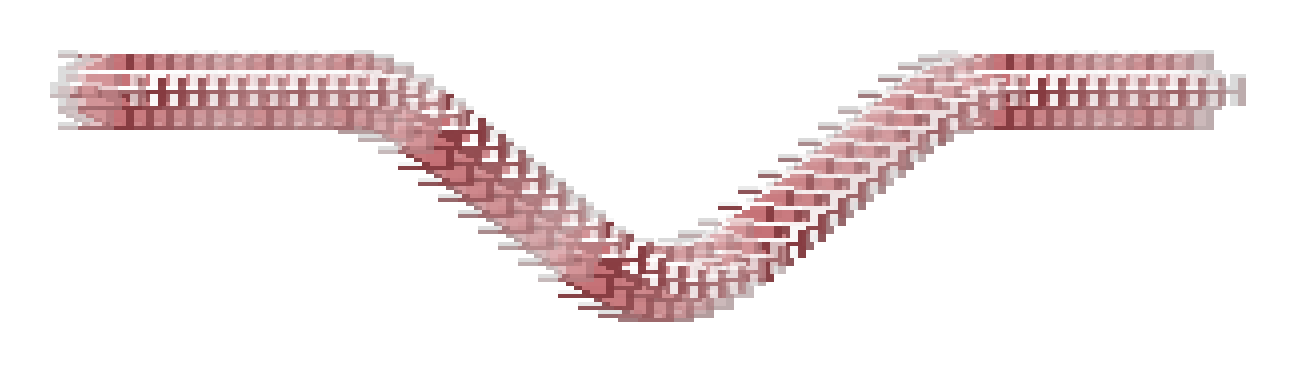
\includegraphics{src/formation_movement/strategies/strategies_1_trimmed.png}%
  \end{adjustbox}
\end{figure}
\vspace{-0.8cm}

Here we have a single enemy progressing from right to left across the screen, dipping down,
then back up, before resuming its forward progress.
The trick to generating this behaviour is to feed the game engine a stream of instructions
that tells it how to alter the \textit{velocity} of the enemy ship over time. For this to
make sense to us, we have to be careful about how we conceptualize \textit{velocity}. We are not just
talking about the speed of the meanie but also, and this is crucial, its direction. 

Think of it this way: at any given time a meanie is considered to have a speed in both the X and the Y directions. 
For example, it could be going at a rate of 5 pixels per frame to the left on the X axis and 3 pixels per frame
downwards on the Y axis. Together, this will generate a \textit{velocity} (a speed and direction)
that is both down and to the left, i.e. on a  diagonal. As we
adjust the speed along each axis we can therefore change not only how quickly the enemy ship is moving, but its direction as well.

To see how this might work, imagine that at some regular interval we subtract
1 from the pixels-per-frame in the ship's downward movement. It will slow down as we reach zero
and when we hit \textit{-1} it will start to change direction. In this way we can alter its
behaviour to go from moving 3 pixels per frame downwards to 3 pixels per frame
upwards. Assuming we have left its movement along the X axis alone,  we can steer the ship from down along a diagonal to moving up along a
diagonal!

Below is an example of the instruction stream used to achieve this precise behaviour in \textit{Uridium}. Each instruction consists of a
pair of bytes. The first byte encodes the directional information. The guidance interpreter will treat an \icode{\$84}
as an instruction to increment the speed in the downward direction, while it will treat \icode{\$88} as an instruction
to increment the speed in the upward direction. In combination with instructions to increment forward movement (\icode{\$82})
and maintain current speed and heading (\icode{\$80}) these provide enough granularity to steer the course of the enemy
ship across the screen. The second byte, as hopefully becomes clear from examining the diagram below, instructs the interpreter
on how long to apply the specified alteration to direction, shaping its path. 

\vspace{-0.5cm}
\begin{minipage}[c]{0.46\linewidth}
	\vspace{-1.9cm}
	\begin{figure}[H]
		\centering
		\begin{adjustbox}{width=7.0cm,right}
			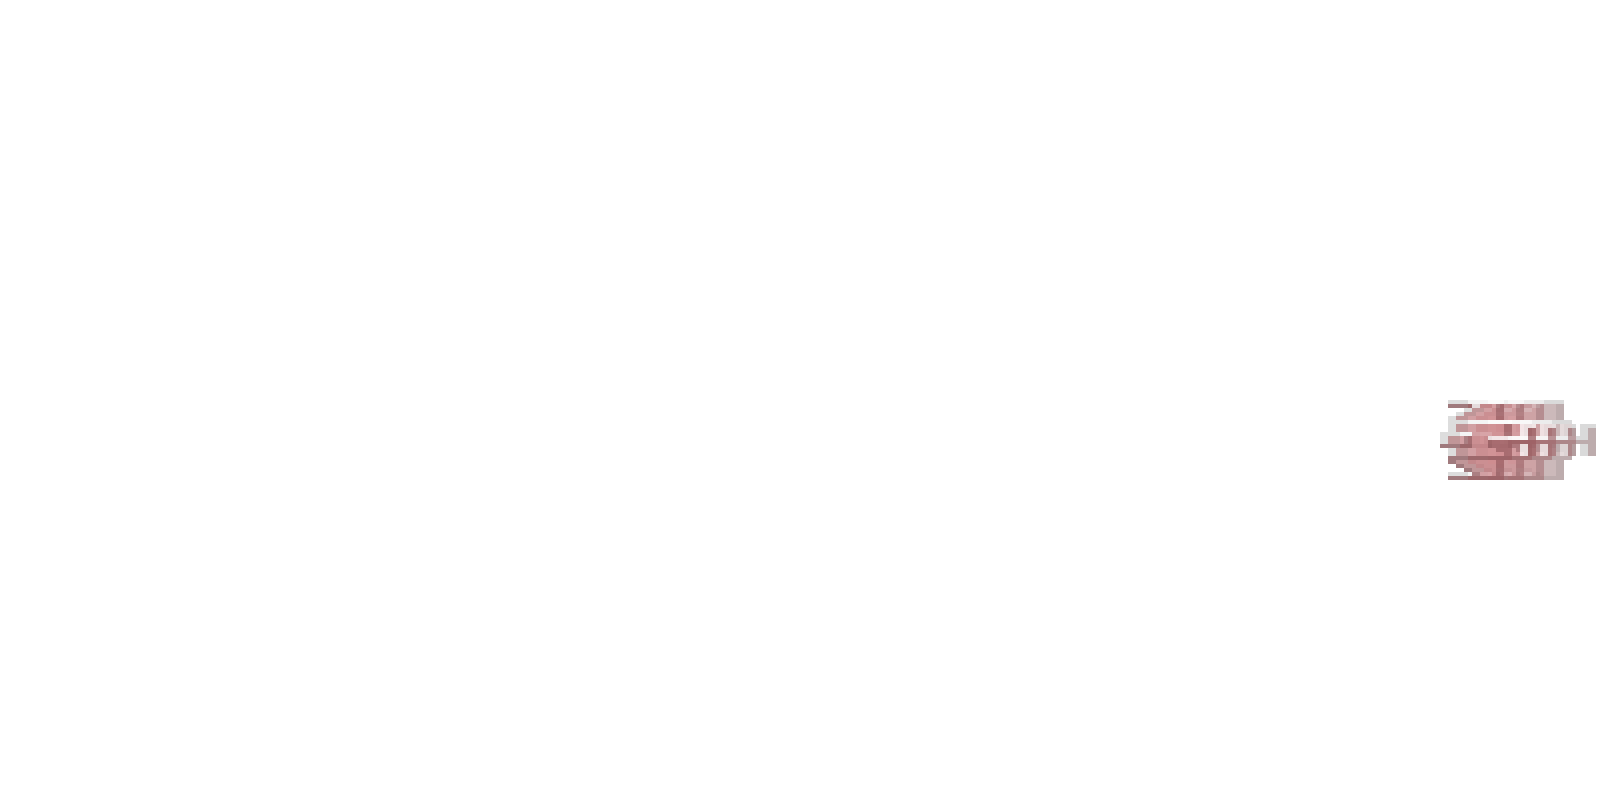
\includegraphics{src/formation_movement/strategies/strategies_1_0.png}%
		\end{adjustbox}
	\end{figure}
	\vspace{-3.3cm}
	\begin{figure}[H]
		\centering
		\begin{adjustbox}{width=7.0cm,right}
			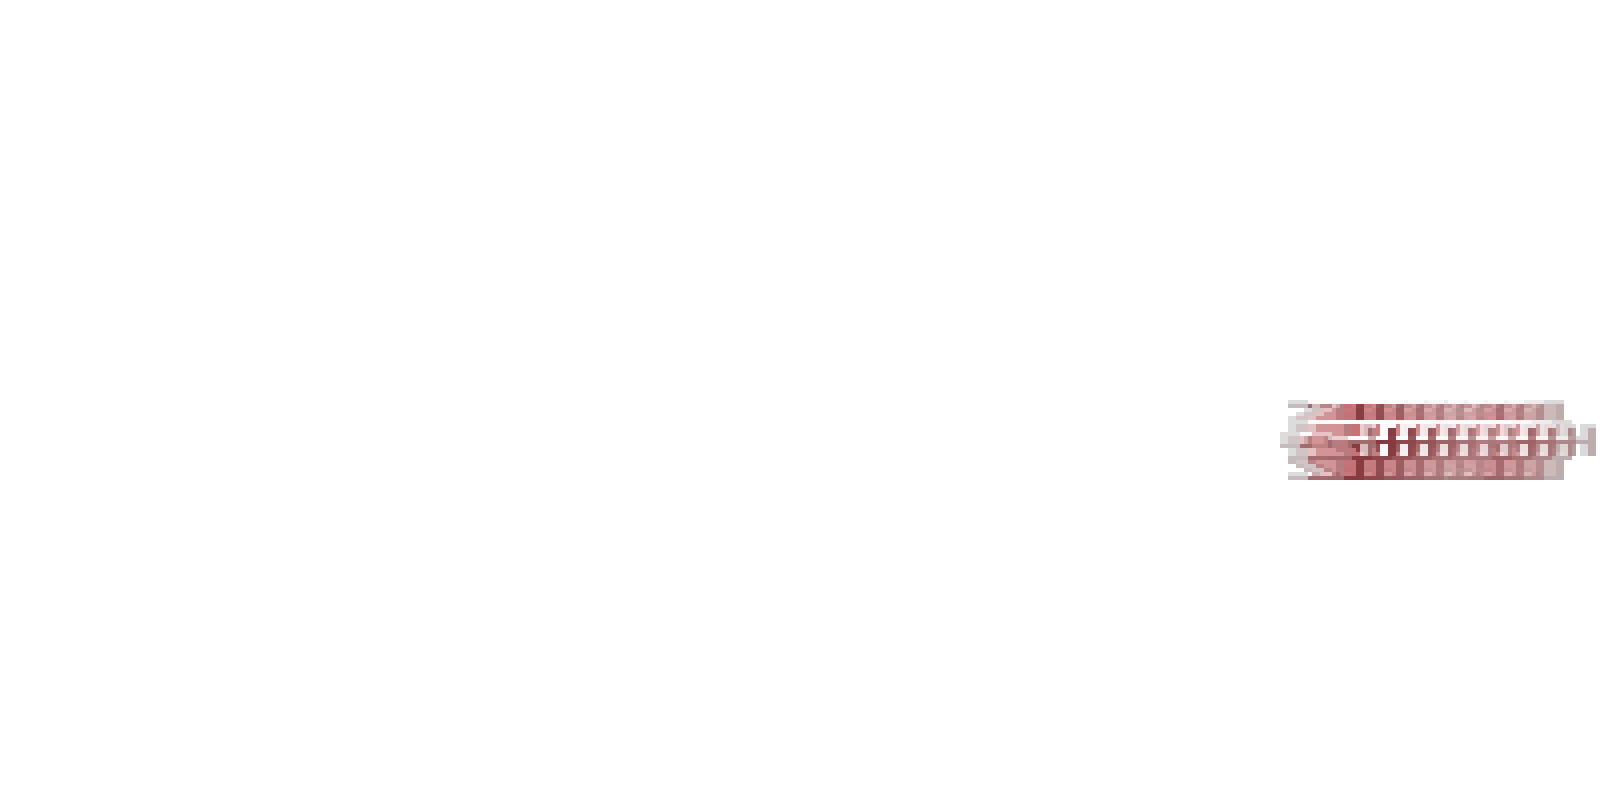
\includegraphics{src/formation_movement/strategies/strategies_1_1.png}%
		\end{adjustbox}
	\end{figure}
	\vspace{-3.3cm}
	\begin{figure}[H]
		\centering
		\begin{adjustbox}{width=7.0cm,right}
			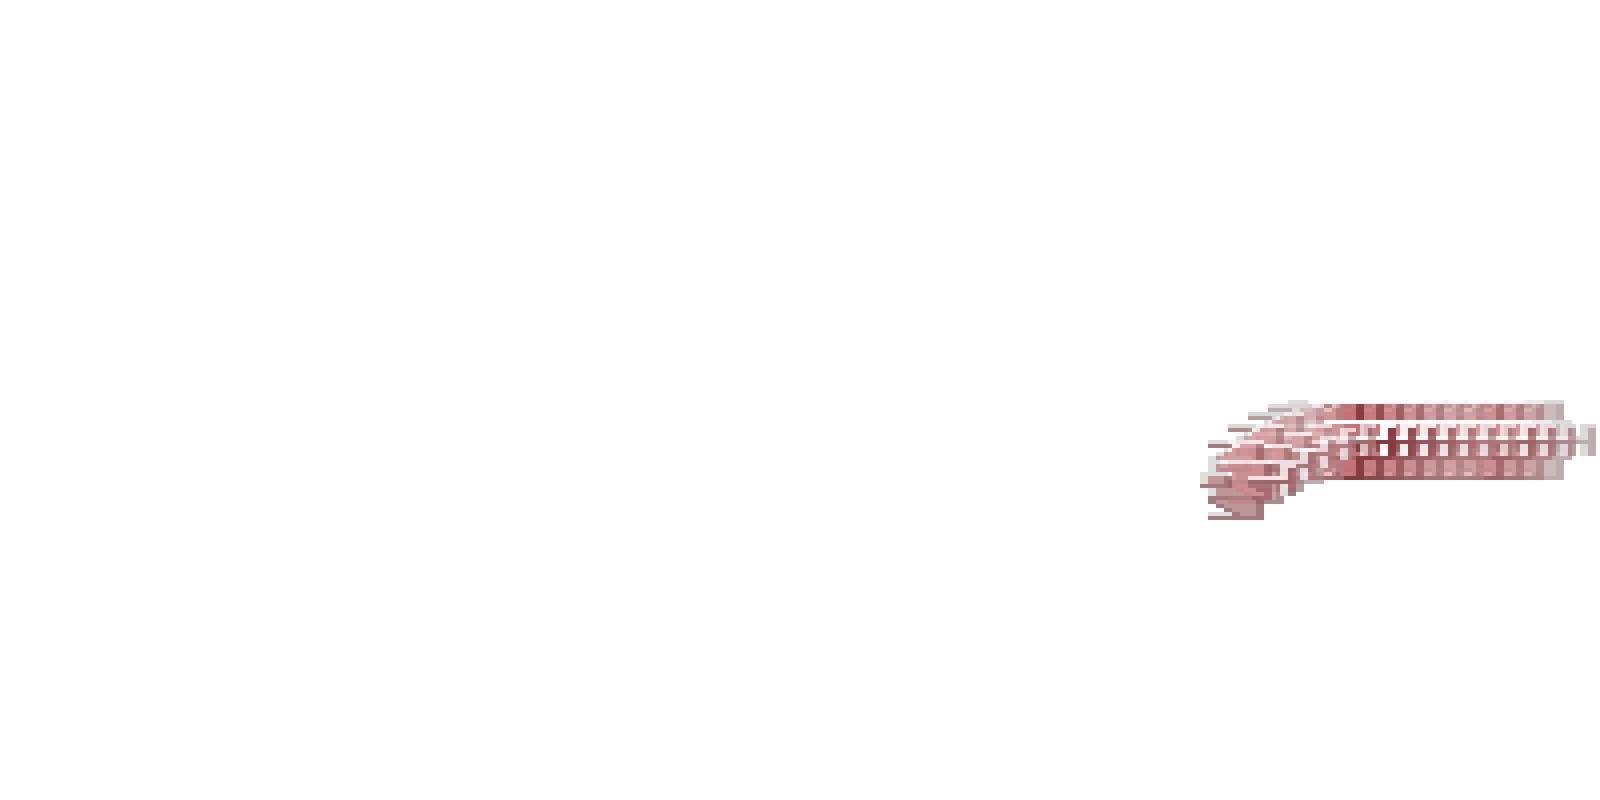
\includegraphics{src/formation_movement/strategies/strategies_1_2.png}%
		\end{adjustbox}
	\end{figure}
	\vspace{-3.3cm}
	\begin{figure}[H]
		\centering
		\begin{adjustbox}{width=7.0cm,right}
			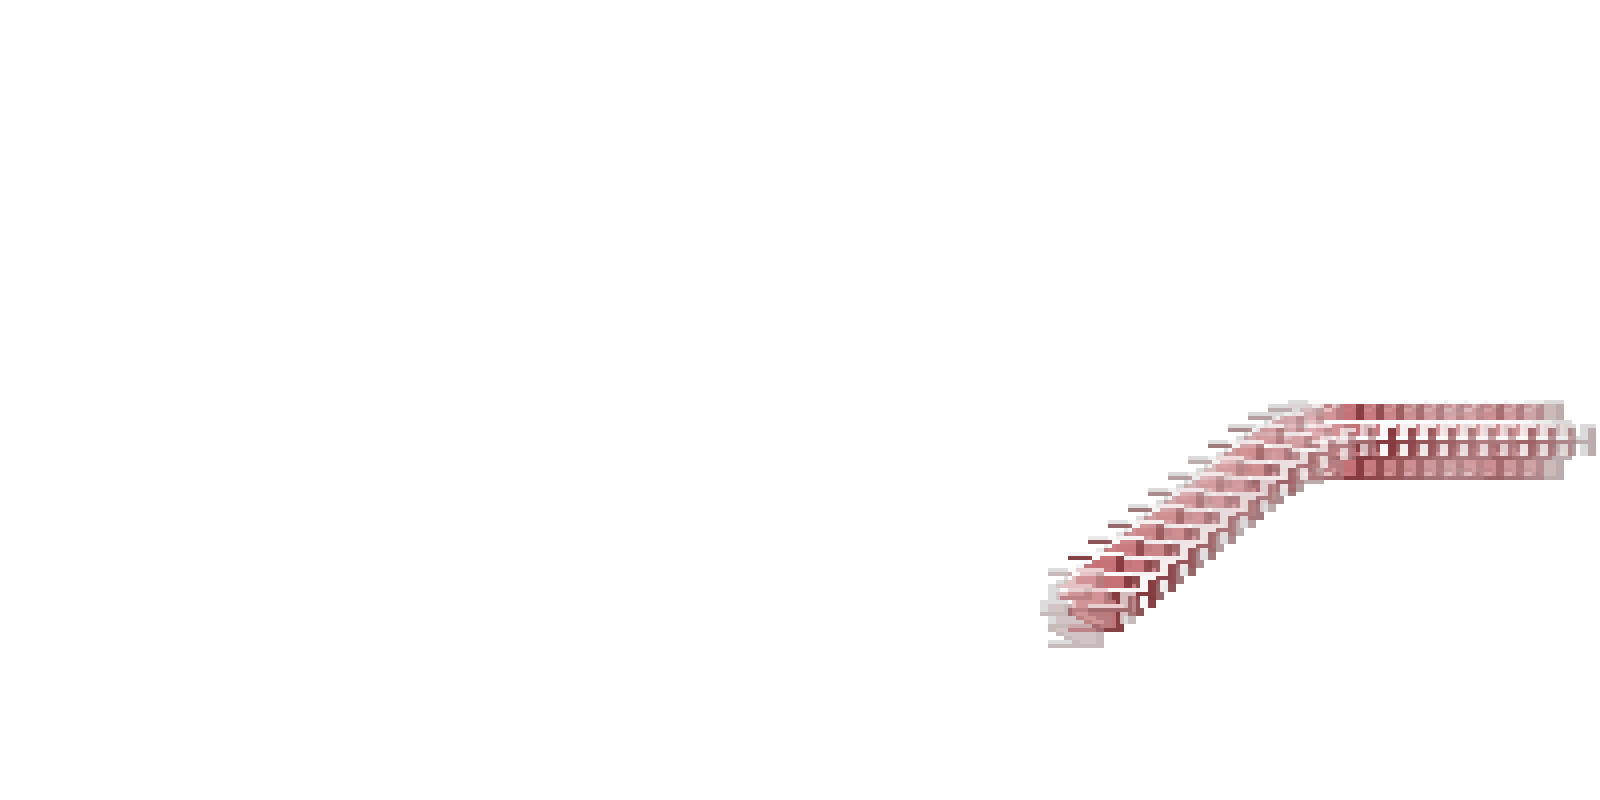
\includegraphics{src/formation_movement/strategies/strategies_1_3.png}%
		\end{adjustbox}
	\end{figure}
	\vspace{-3.3cm}
	\begin{figure}[H]
		\centering
		\begin{adjustbox}{width=7.0cm,right}
			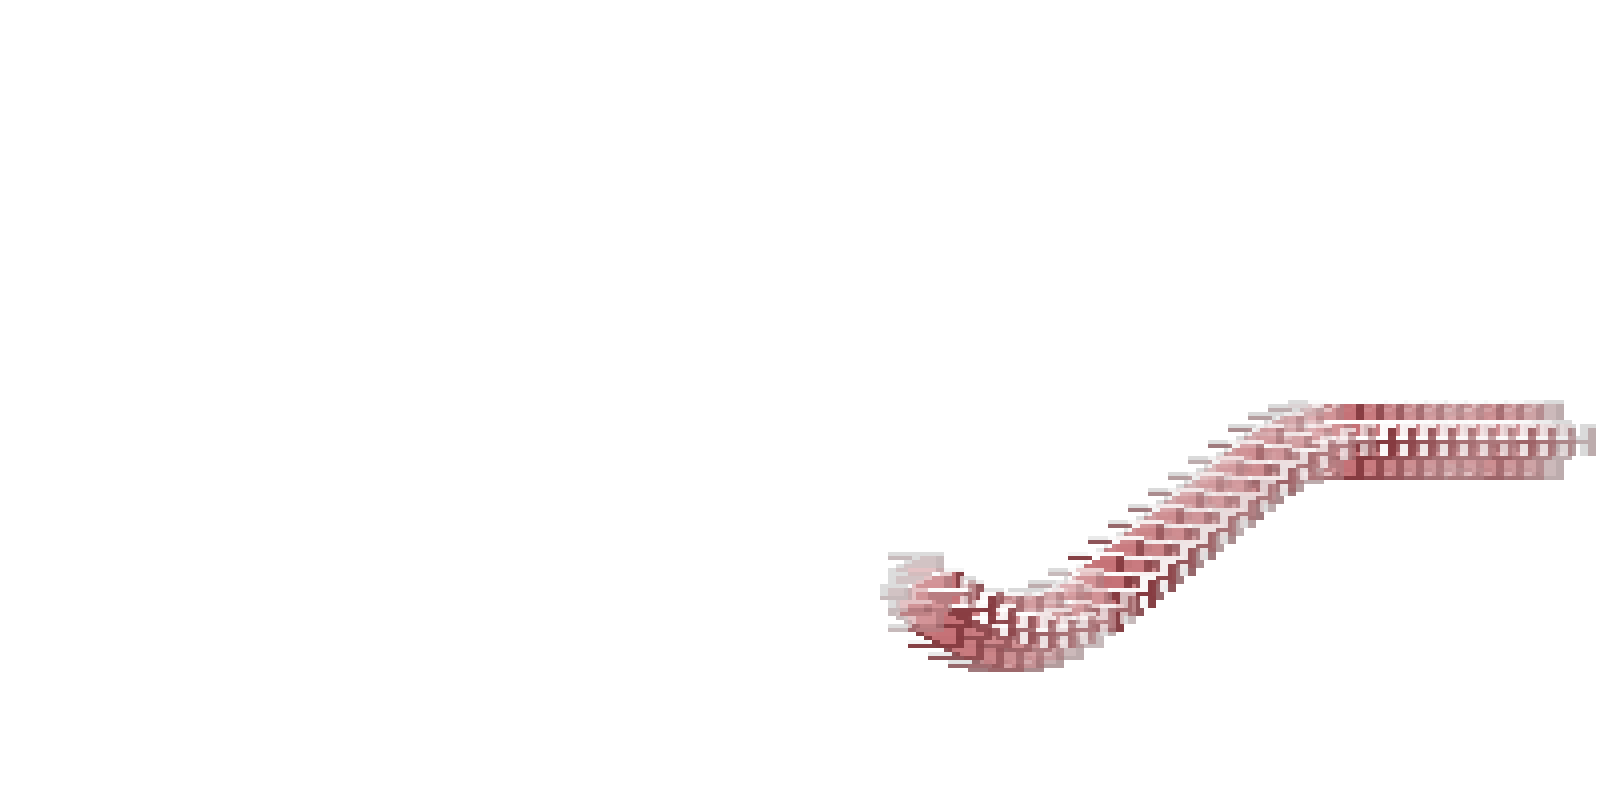
\includegraphics{src/formation_movement/strategies/strategies_1_4.png}%
		\end{adjustbox}
	\end{figure}
	\vspace{-3.4cm}
	\begin{figure}[H]
		\centering
		\begin{adjustbox}{width=7.0cm,right}
			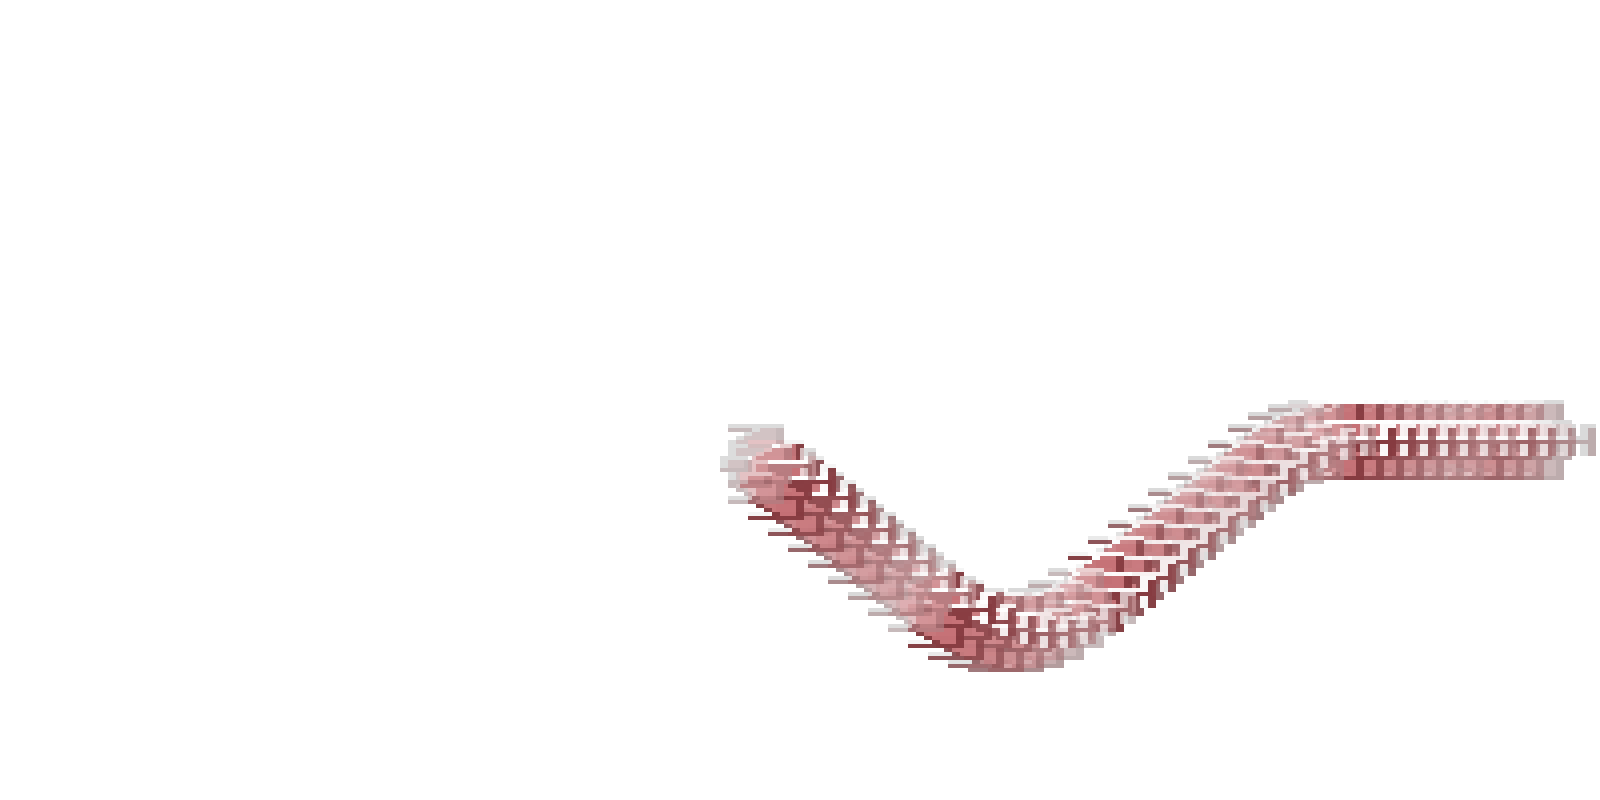
\includegraphics{src/formation_movement/strategies/strategies_1_5.png}%
		\end{adjustbox}
	\end{figure}
	\vspace{-3.4cm}
	\begin{figure}[H]
		\centering
		\begin{adjustbox}{width=7.0cm,right}
			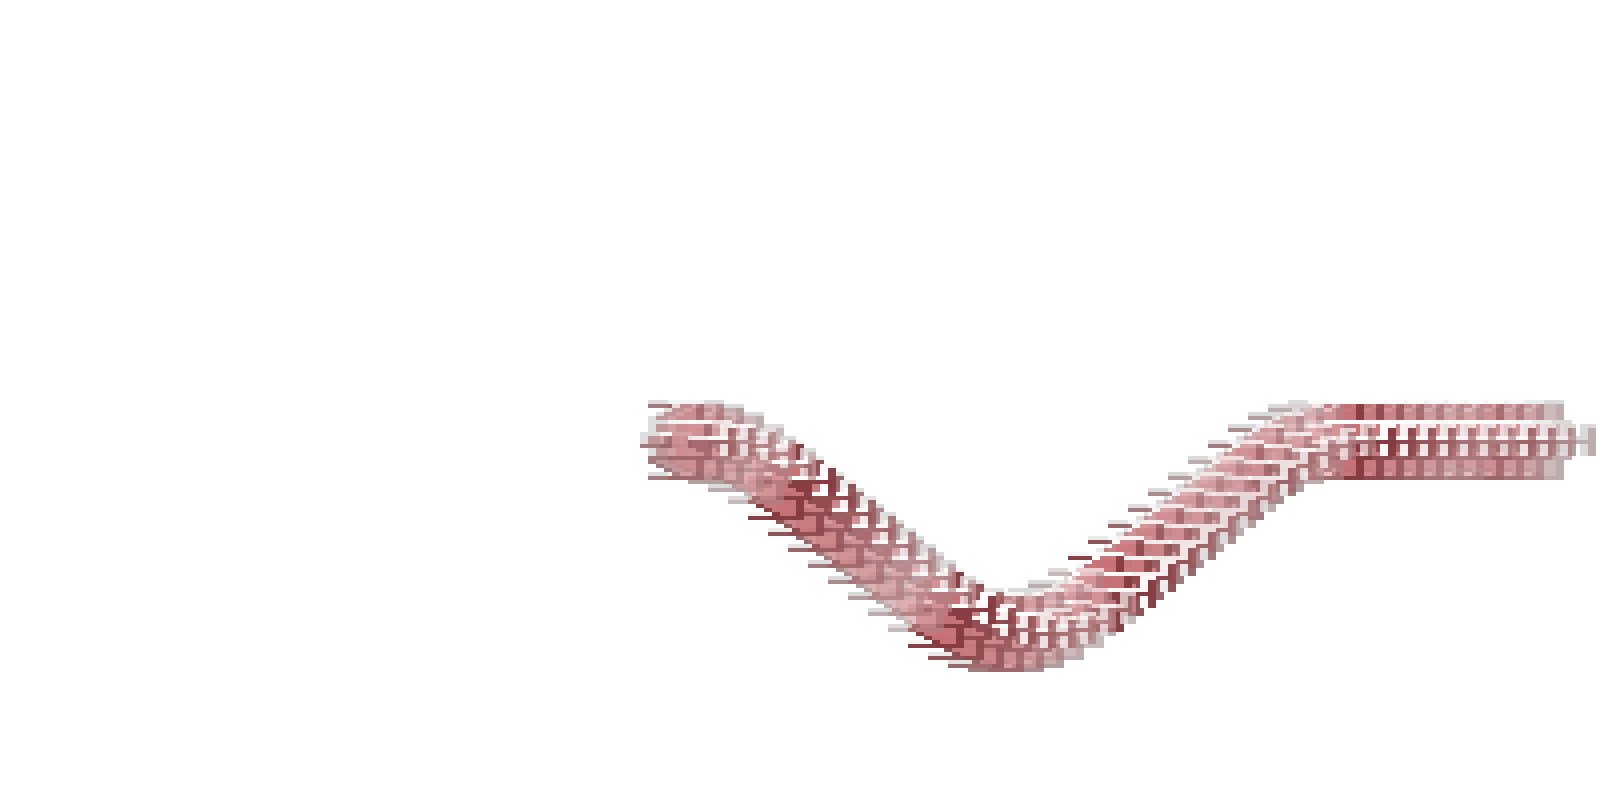
\includegraphics{src/formation_movement/strategies/strategies_1_6.png}%
		\end{adjustbox}
	\end{figure}
	\vspace{-3.4cm}
	\begin{figure}[H]
		\centering
		\begin{adjustbox}{width=7.0cm,right}
			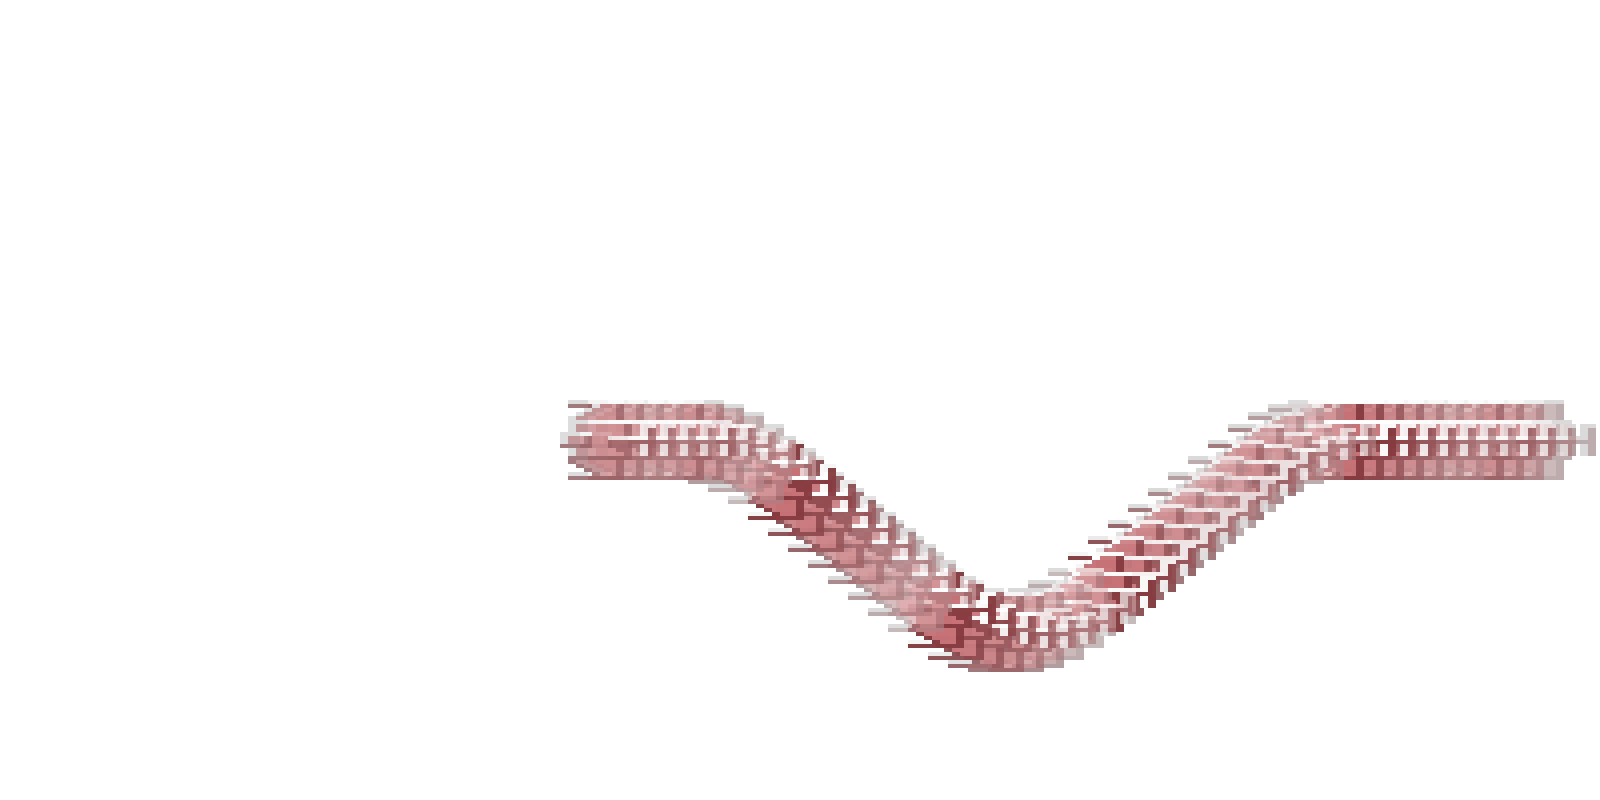
\includegraphics{src/formation_movement/strategies/strategies_1_7.png}%
		\end{adjustbox}
	\end{figure}
	\vspace{-3.4cm}
	\begin{figure}[H]
		\centering
		\begin{adjustbox}{width=7.0cm,right}
			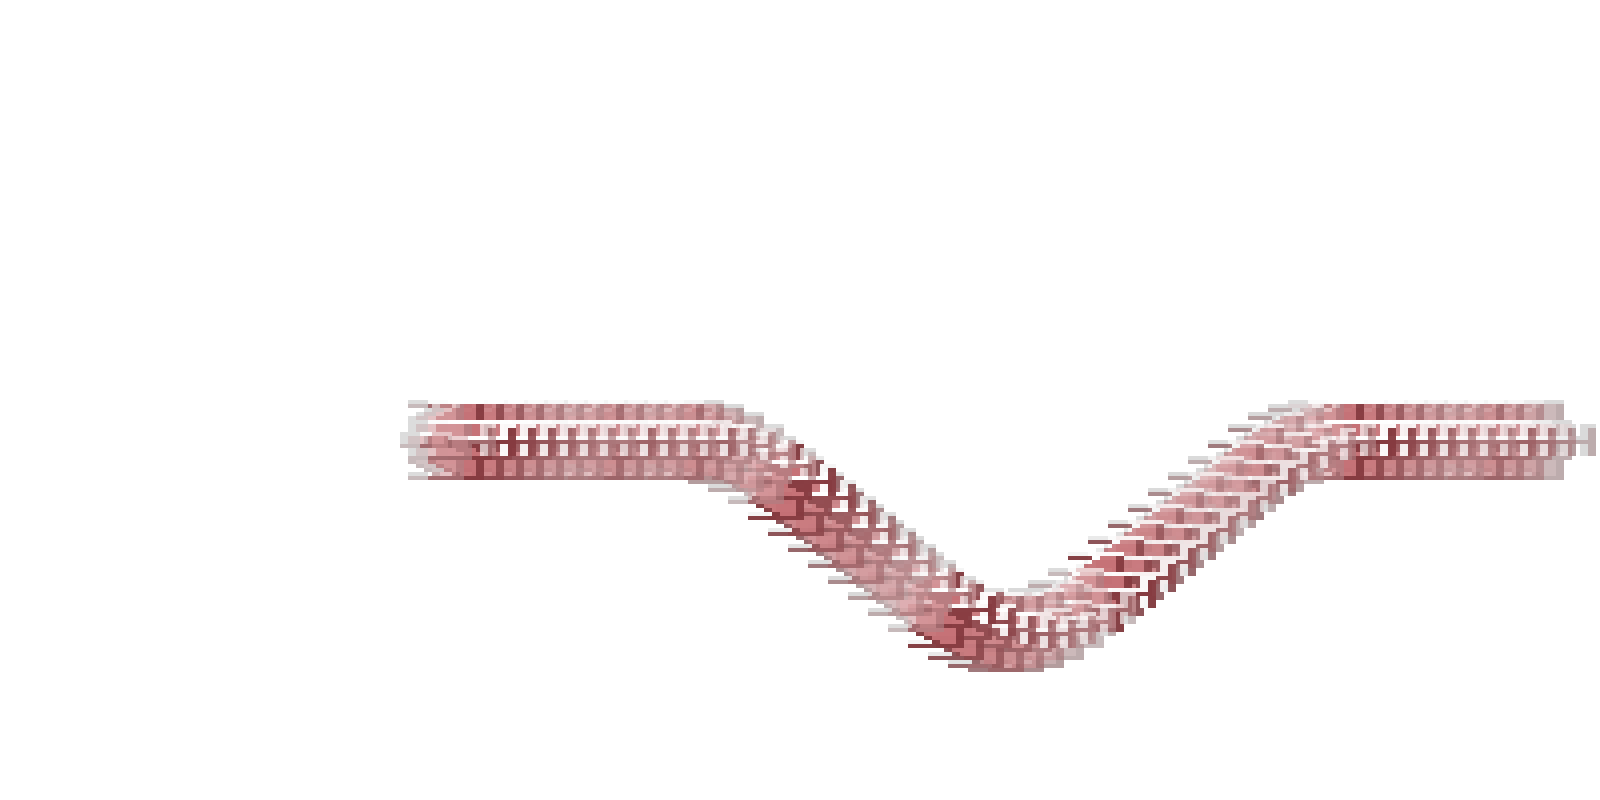
\includegraphics{src/formation_movement/strategies/strategies_1_8.png}%
		\end{adjustbox}
	\end{figure}
\end{minipage}
\hspace{0.2cm}
\begin{minipage}[c]{0.48\linewidth}
	\vspace{-1.0cm}
\begin{lstlisting}[basicstyle=\footnotesize\ttfamily]
.BYTE $82 ; Move forward.
.BYTE $08 ; Repeat for 8 ticks.

.BYTE $80 ; Maintain movement.
.BYTE $10 ; Repeat for 16 ticks.

.BYTE $84 ; Move down .
.BYTE $08 ; 8 ticks.

.BYTE $80 ; Maintain movement.
.BYTE $10 ; 16 ticks.

.BYTE $88 ; Move up.
.BYTE $10 ; 16 ticks.

.BYTE $80 ; Maintain movement..
.BYTE $10 ; 16 ticks.

.BYTE $84 ; Move down
.BYTE $08 ; 8 ticks.

.BYTE $82 ; Move forward.
.BYTE $08 ; 8 ticks.

.BYTE $00
.BYTE $FF ; Terminal pair.
\end{lstlisting}
\end{minipage}
\vspace{-0.6cm}

Notice how the length of each new segment in the path is dependent on the value given in the second
byte. And notice how the directional nudge applied by the first byte in each pair acts progressively, rather
than immediately, on the velocity of the ship. At all times our instructions are acting on the enemy's existing inertial
velocity, gradually\linebreak

\begin{minipage}[c]{0.46\linewidth}
	\vspace{-2.6cm}
	\begin{figure}[H]
		\centering
		\begin{adjustbox}{width=7.0cm,right}
			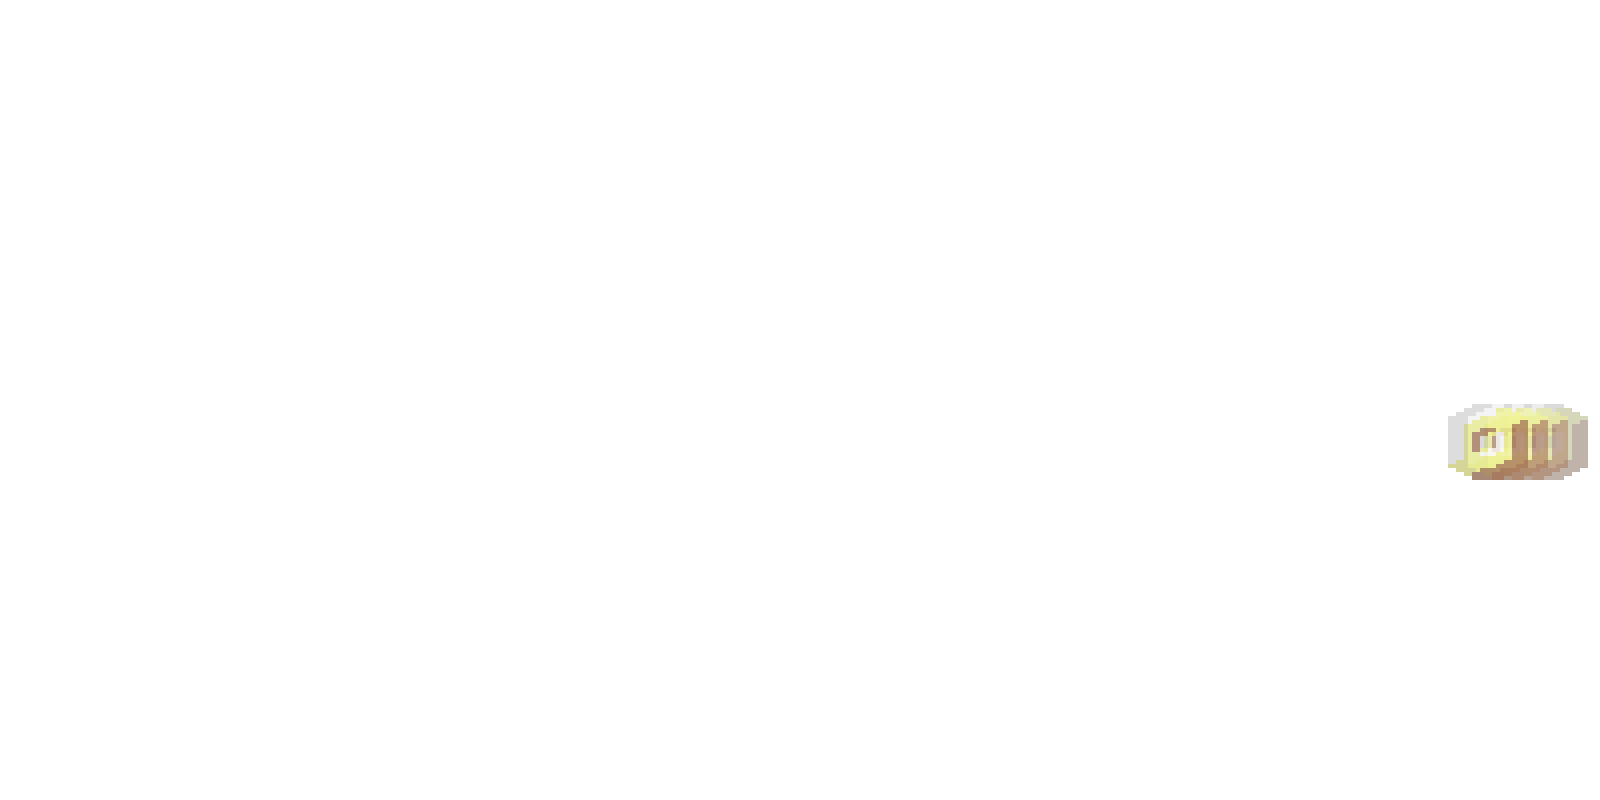
\includegraphics{src/formation_movement/strategies/strategies_17_0.png}%
		\end{adjustbox}
	\end{figure}
	\vspace{-3.3cm}
	\begin{figure}[H]
		\centering
		\begin{adjustbox}{width=7.0cm,right}
			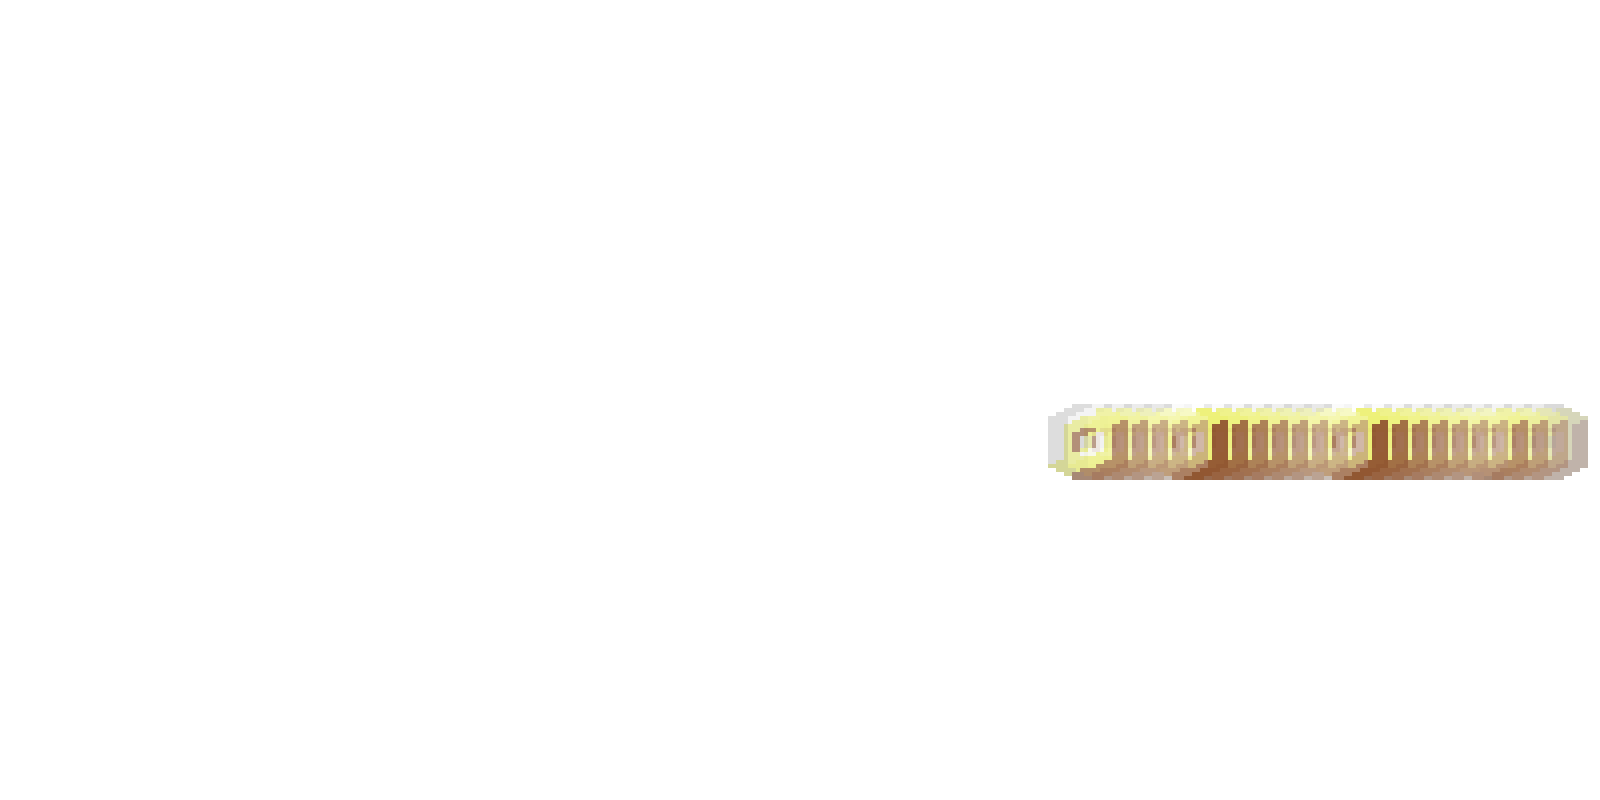
\includegraphics{src/formation_movement/strategies/strategies_17_1.png}%
		\end{adjustbox}
	\end{figure}
	\vspace{-3.3cm}
	\begin{figure}[H]
		\centering
		\begin{adjustbox}{width=7.0cm,right}
			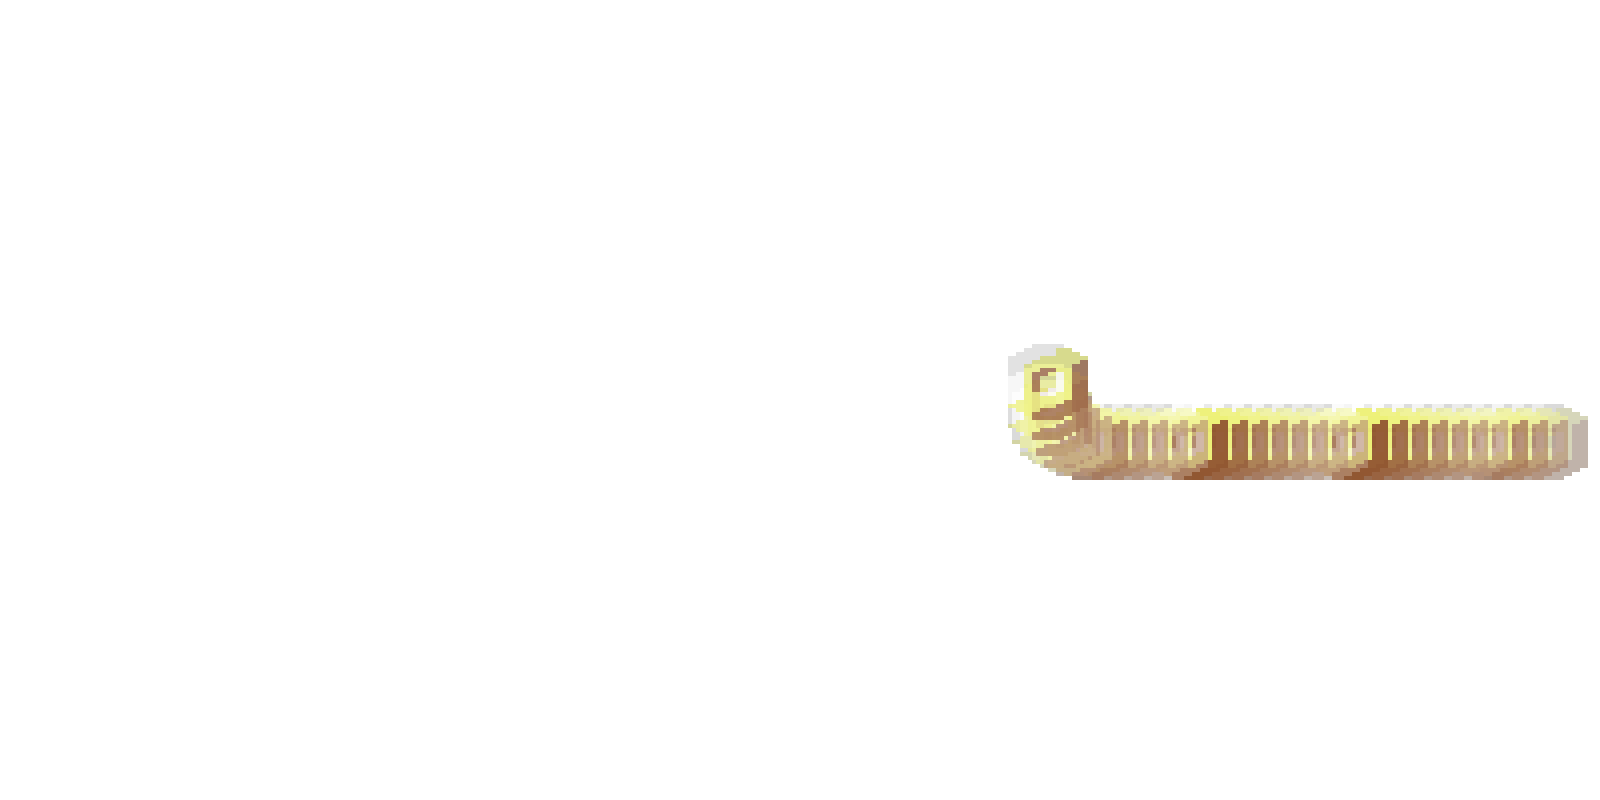
\includegraphics{src/formation_movement/strategies/strategies_17_2.png}%
		\end{adjustbox}
	\end{figure}
	\vspace{-3.3cm}
	\begin{figure}[H]
		\centering
		\begin{adjustbox}{width=7.0cm,right}
			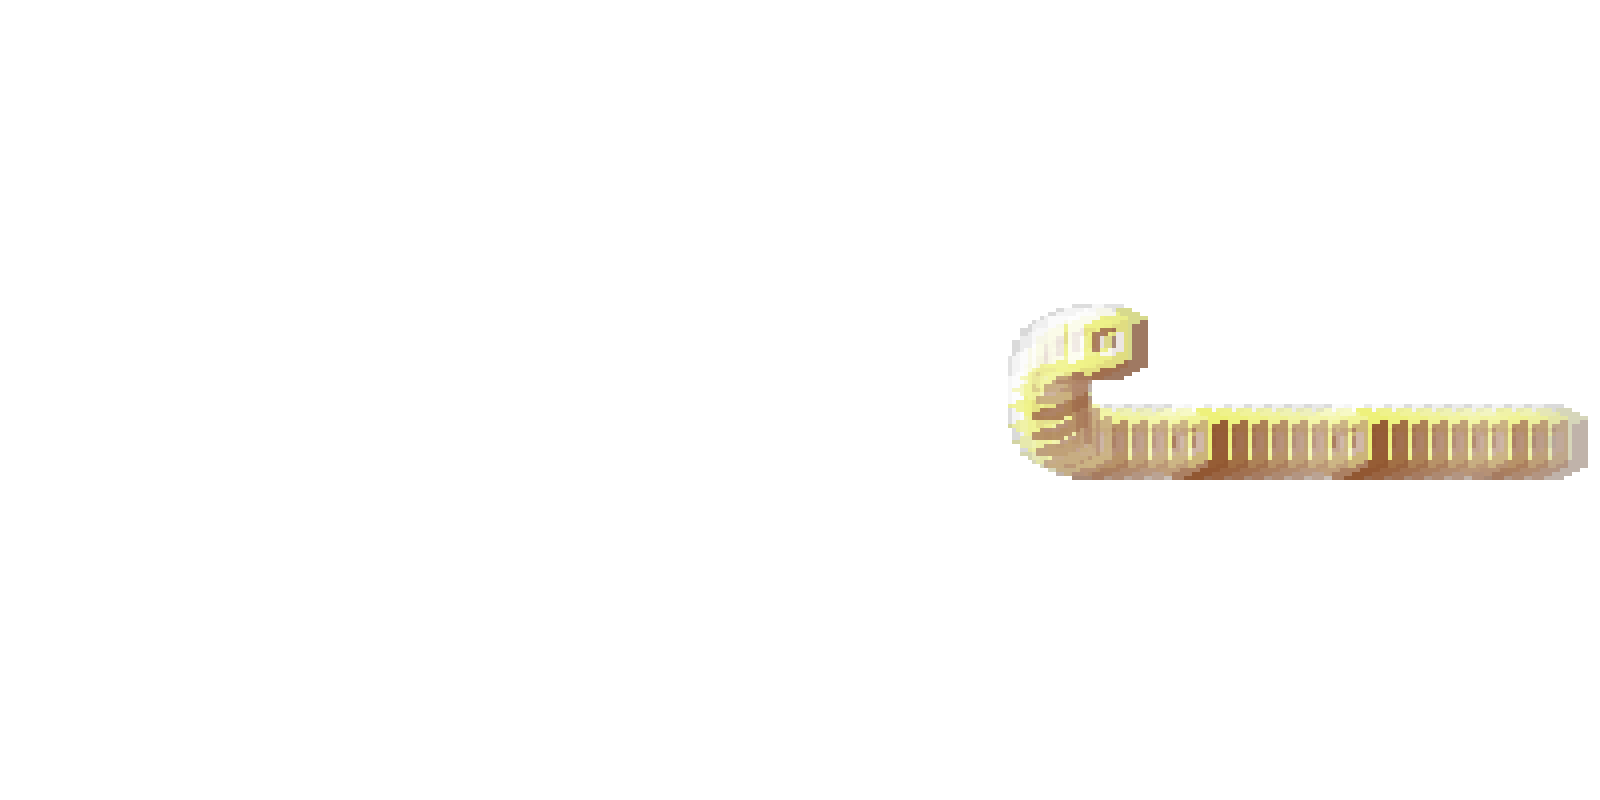
\includegraphics{src/formation_movement/strategies/strategies_17_3.png}%
		\end{adjustbox}
	\end{figure}
	\vspace{-3.3cm}
	\begin{figure}[H]
		\centering
		\begin{adjustbox}{width=7.0cm,right}
			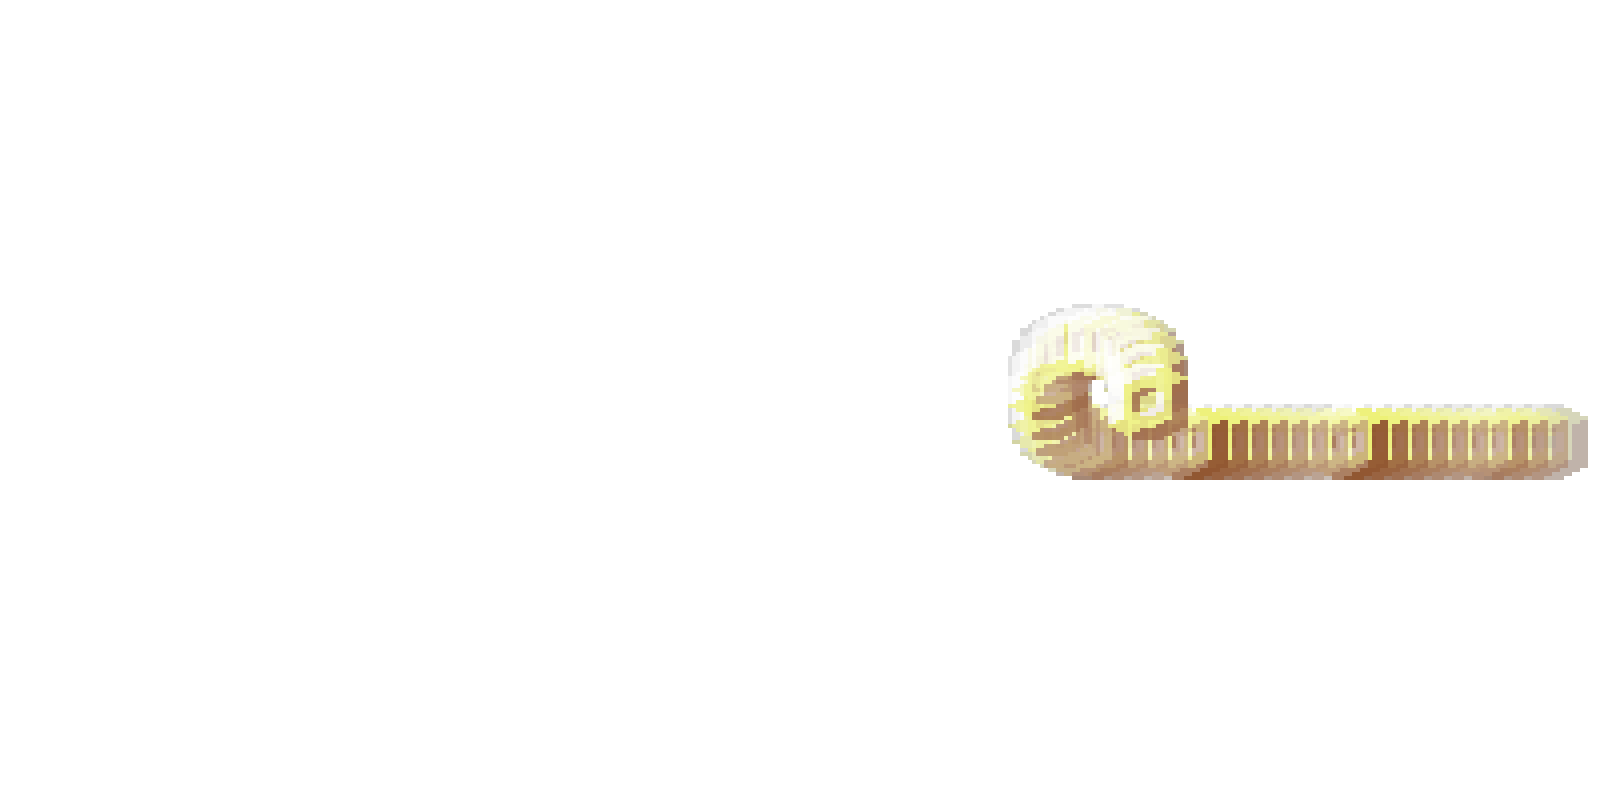
\includegraphics{src/formation_movement/strategies/strategies_17_4.png}%
		\end{adjustbox}
	\end{figure}
	\vspace{-3.2cm}
	\begin{figure}[H]
		\centering
		\begin{adjustbox}{width=7.0cm,right}
			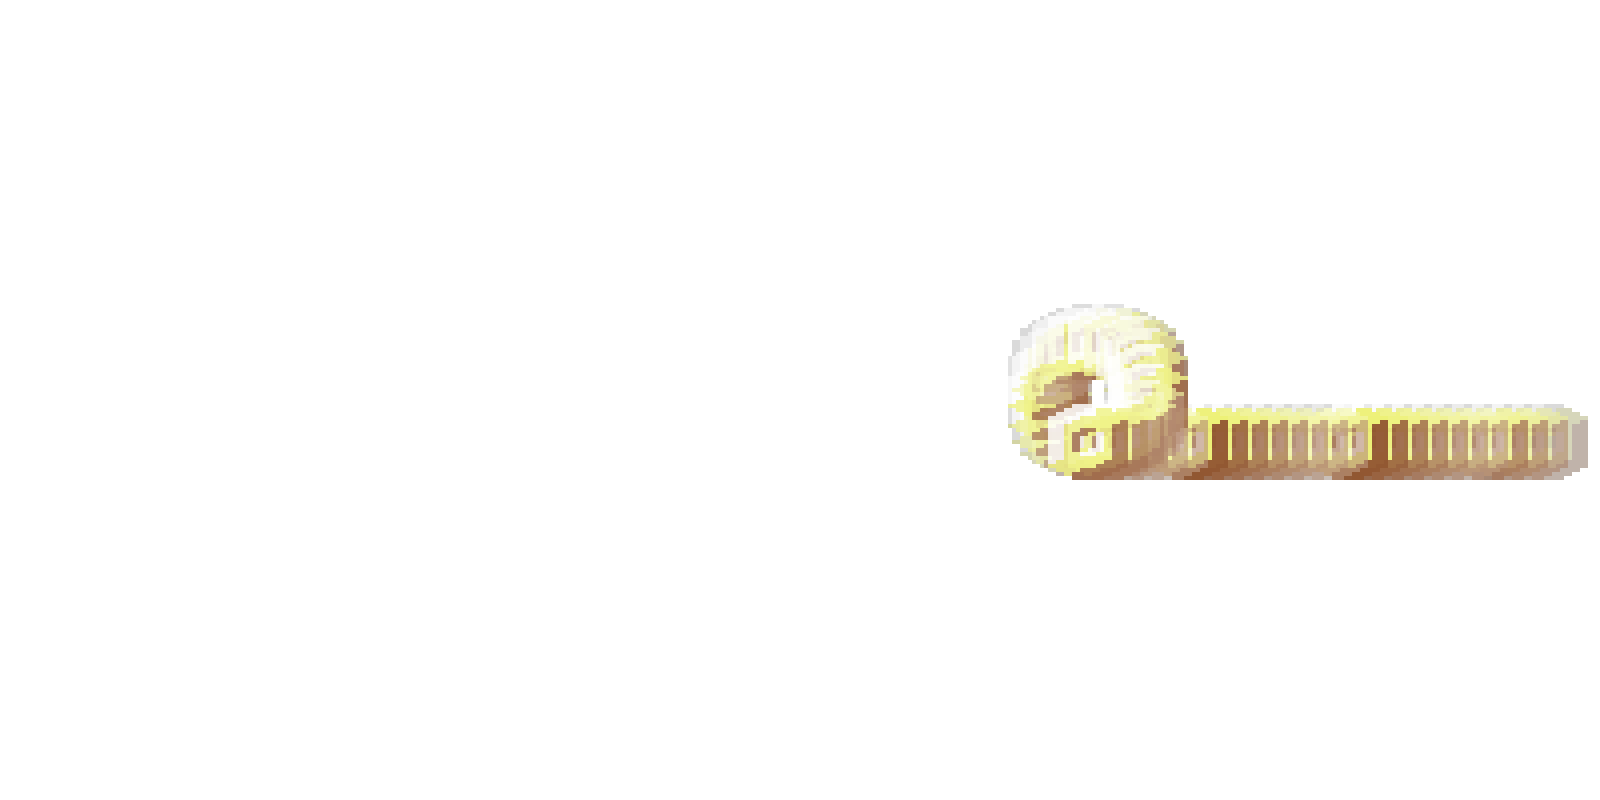
\includegraphics{src/formation_movement/strategies/strategies_17_5.png}%
		\end{adjustbox}
	\end{figure}
	\vspace{-3.4cm}
	\begin{figure}[H]
		\centering
		\begin{adjustbox}{width=7.0cm,right}
			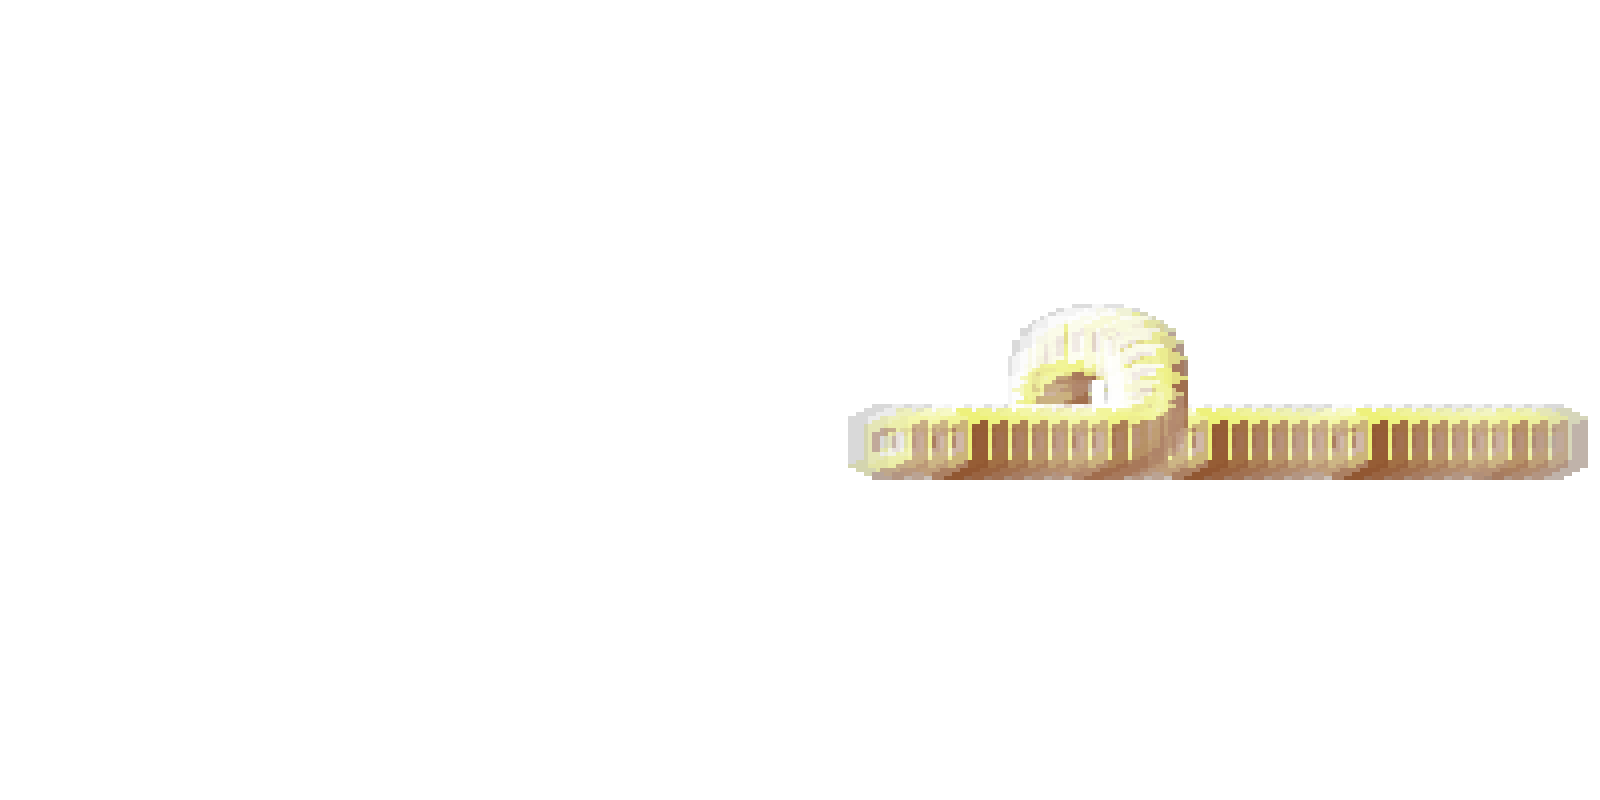
\includegraphics{src/formation_movement/strategies/strategies_17_6.png}%
		\end{adjustbox}
	\end{figure}
	\vspace{-3.4cm}
	\begin{figure}[H]
		\centering
		\begin{adjustbox}{width=7.0cm,right}
			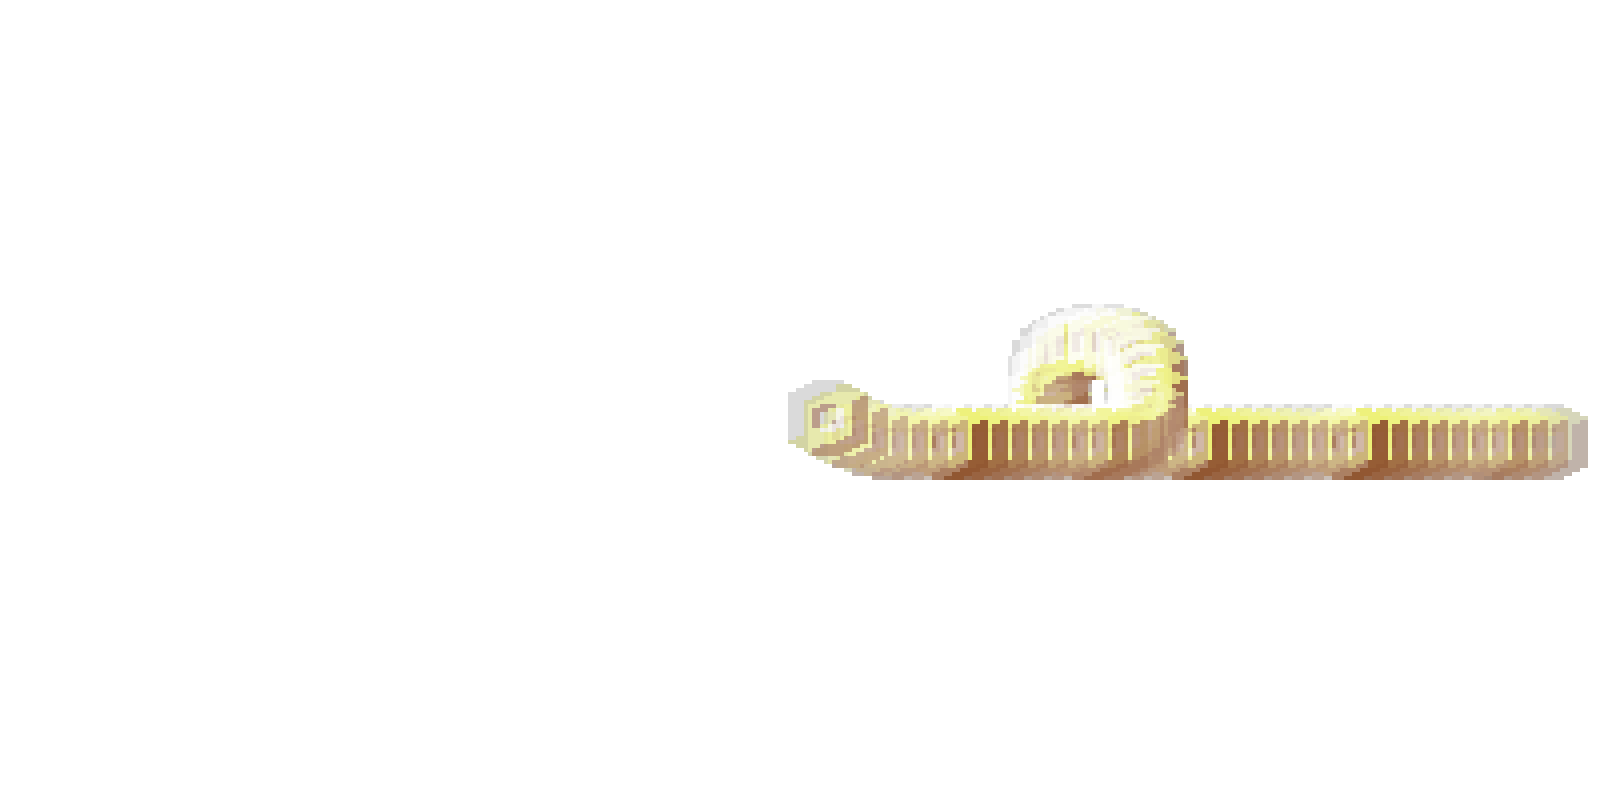
\includegraphics{src/formation_movement/strategies/strategies_17_7.png}%
		\end{adjustbox}
	\end{figure}
	\vspace{-3.4cm}
	\begin{figure}[H]
		\centering
		\begin{adjustbox}{width=7.0cm,right}
			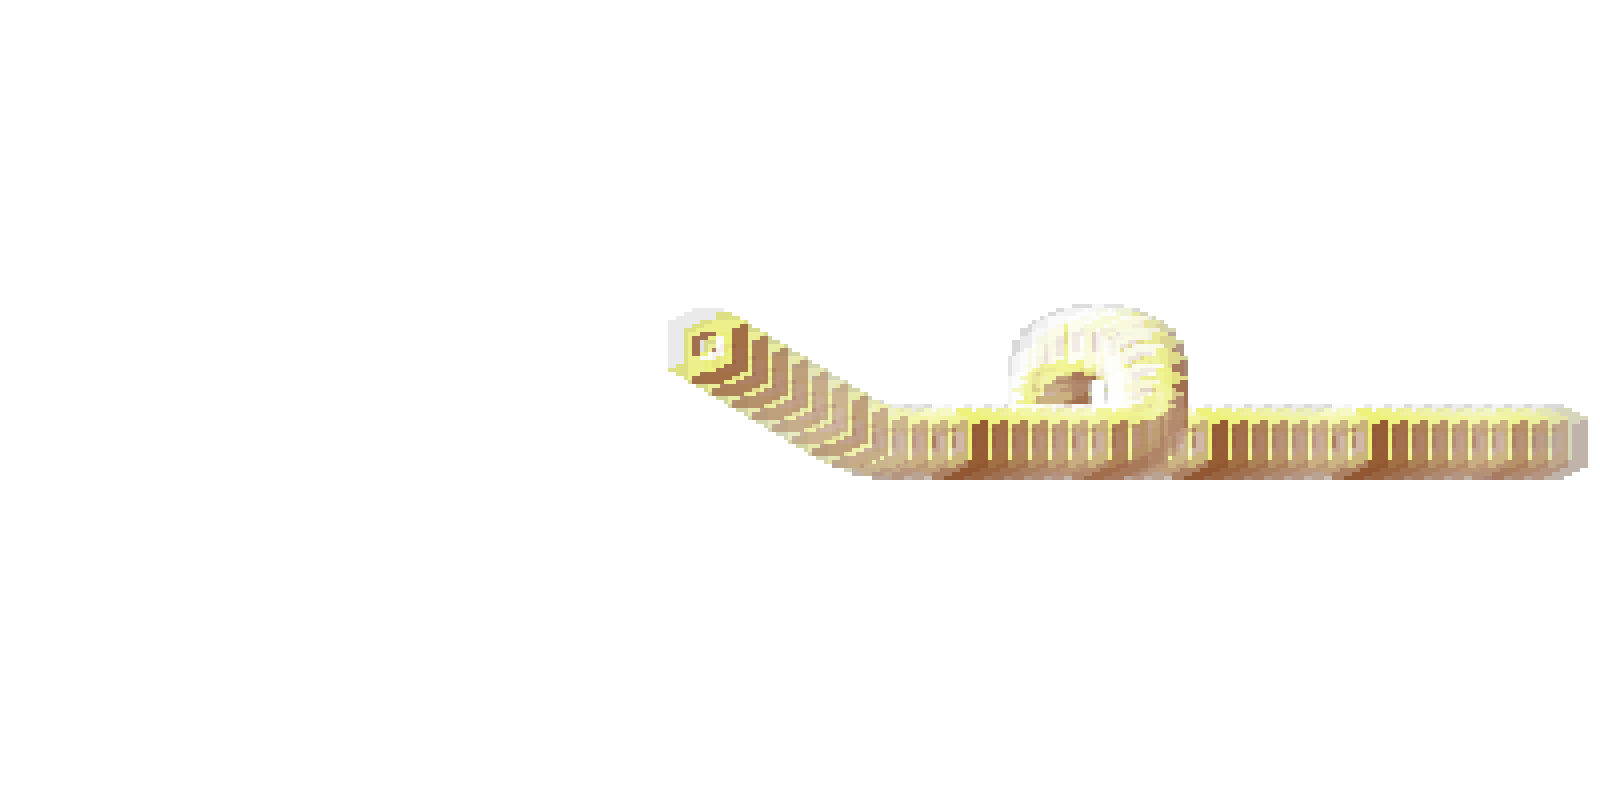
\includegraphics{src/formation_movement/strategies/strategies_17_8.png}%
		\end{adjustbox}
	\end{figure}
	\vspace{-3.4cm}
	\begin{figure}[H]
		\centering
		\begin{adjustbox}{width=7.0cm,right}
			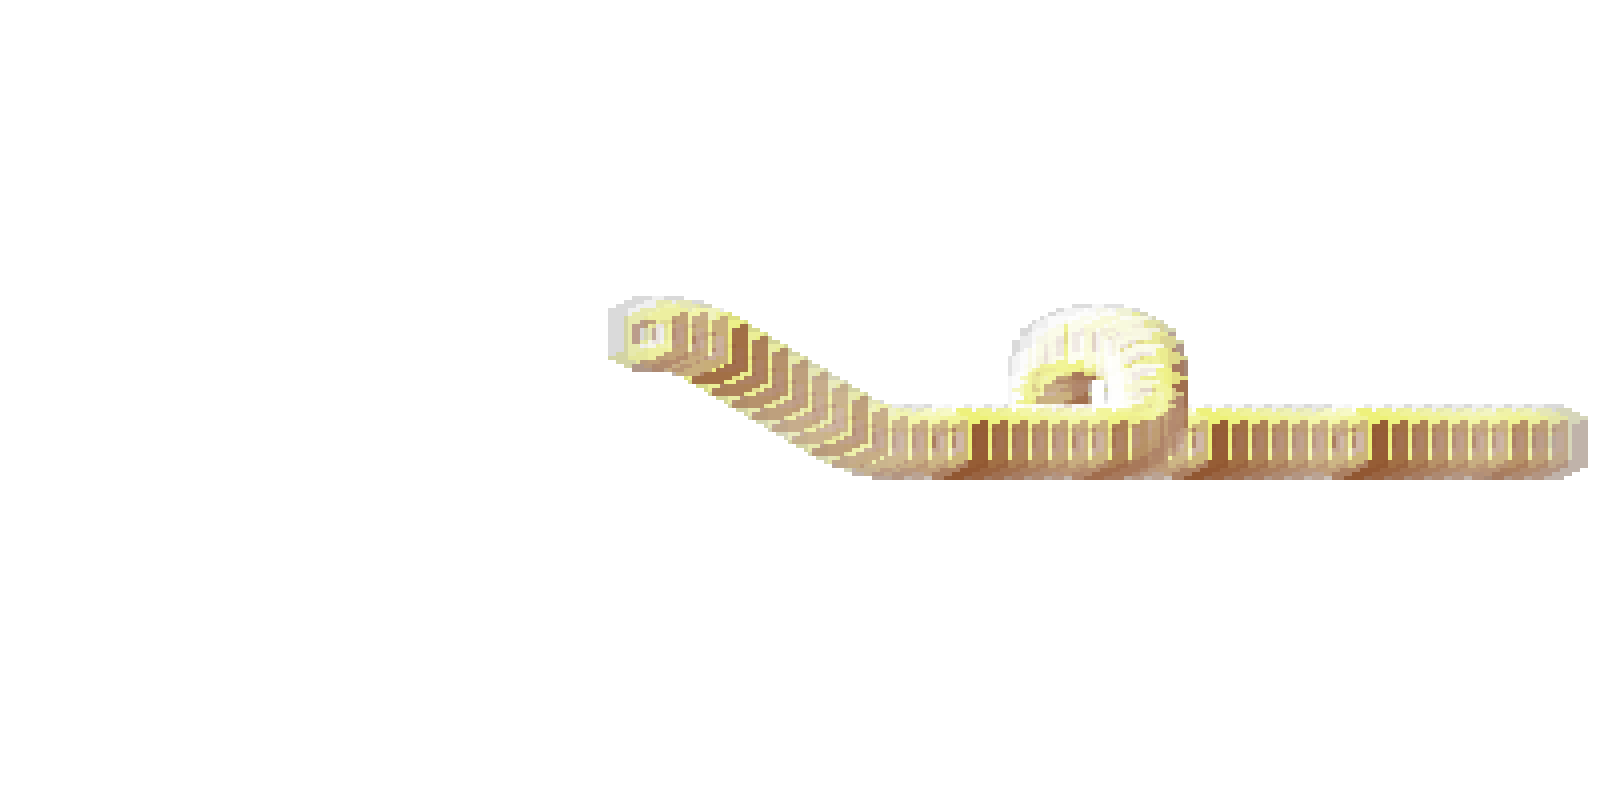
\includegraphics{src/formation_movement/strategies/strategies_17_9.png}%
		\end{adjustbox}
	\end{figure}
	\vspace{-3.4cm}
	\begin{figure}[H]
		\centering
		\begin{adjustbox}{width=7.0cm,right}
			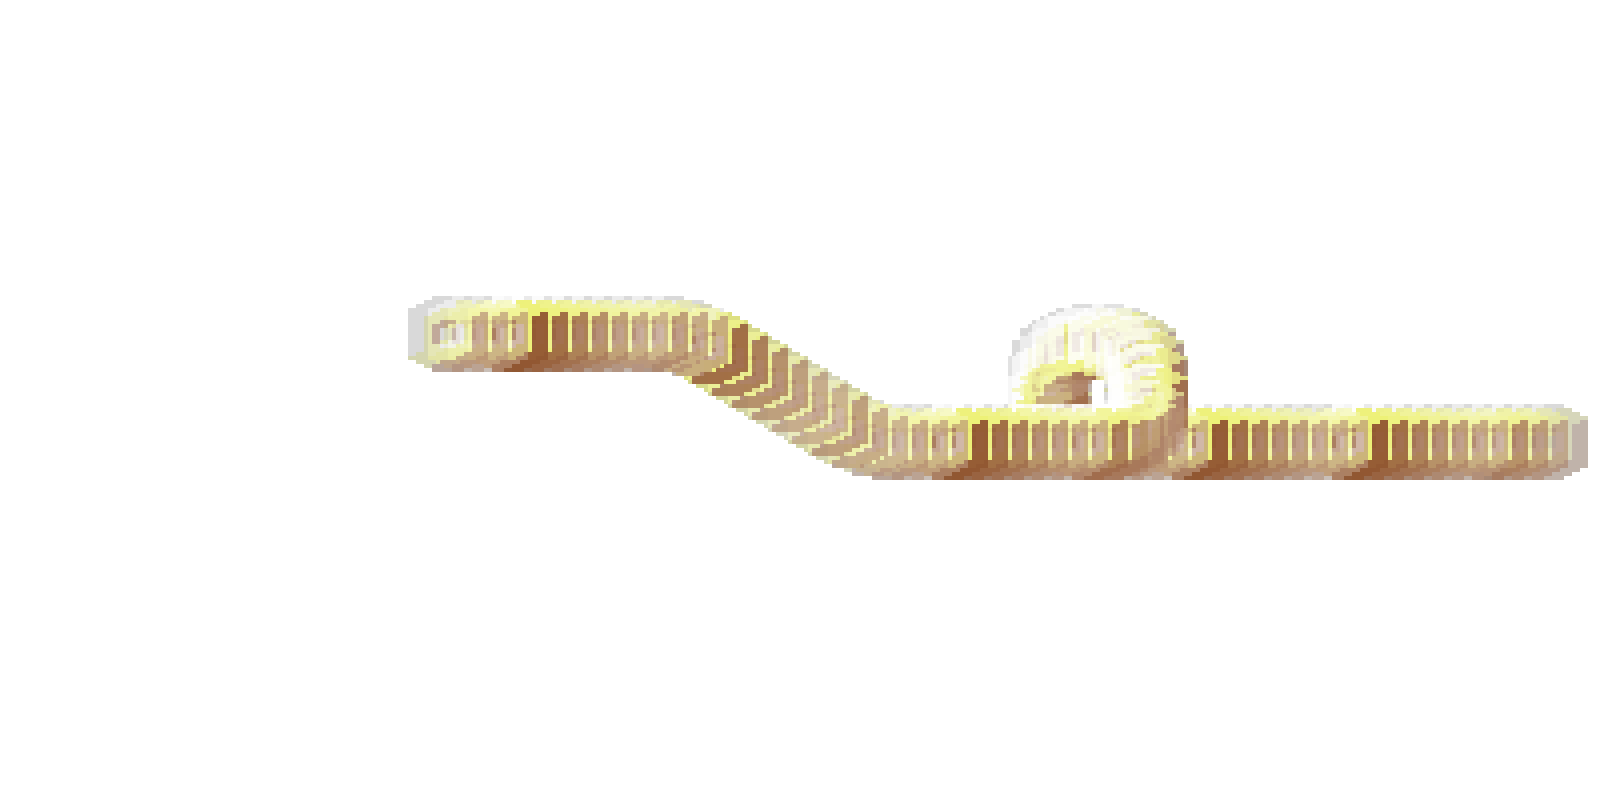
\includegraphics{src/formation_movement/strategies/strategies_17_10.png}%
		\end{adjustbox}
	\end{figure}
	\vspace{-3.4cm}
	\begin{figure}[H]
		\centering
		\begin{adjustbox}{width=7.0cm,right}
			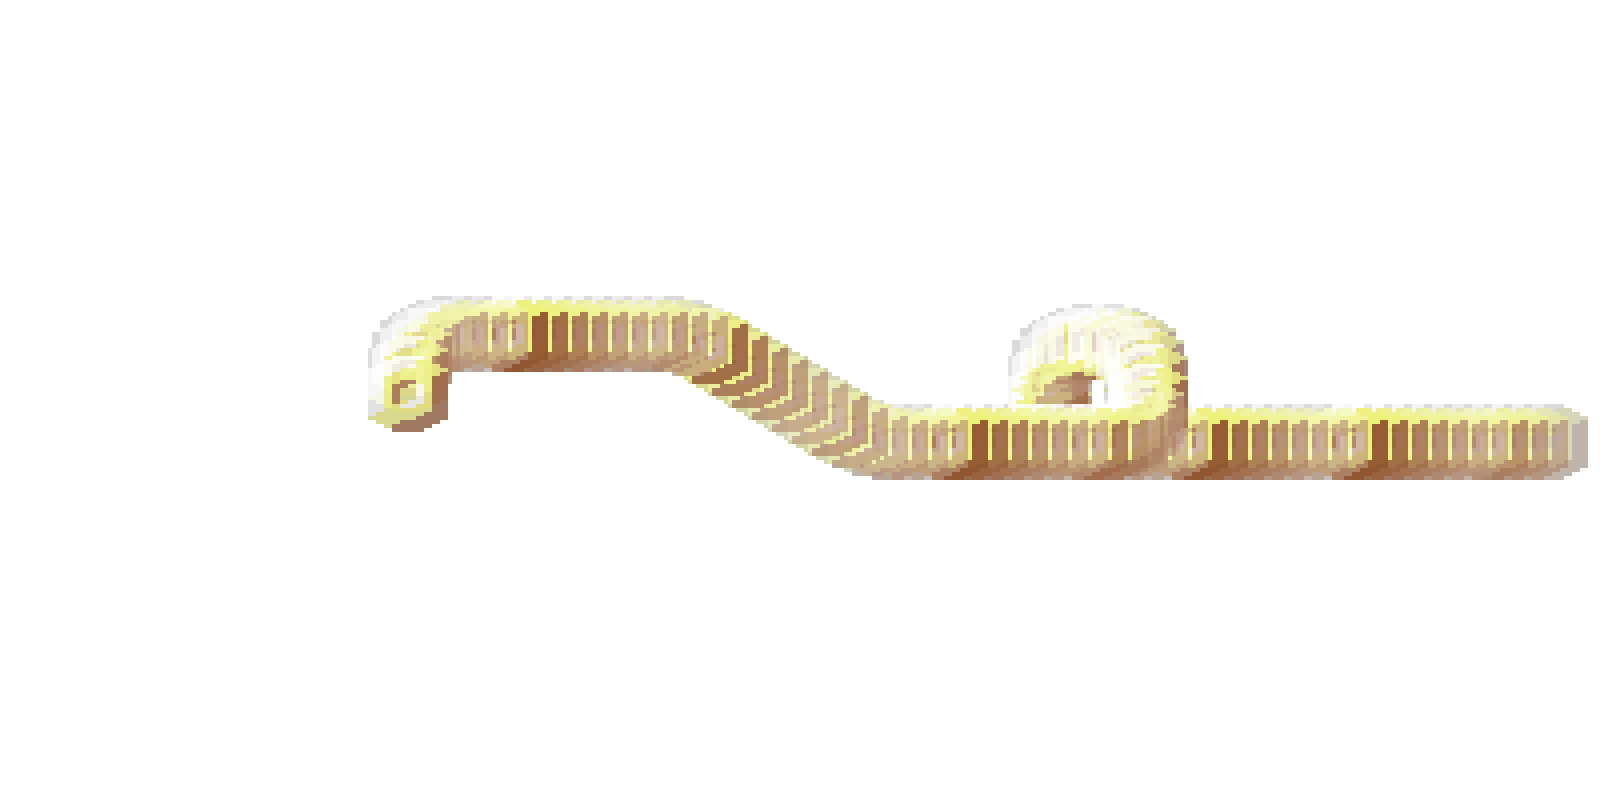
\includegraphics{src/formation_movement/strategies/strategies_17_11.png}%
		\end{adjustbox}
	\end{figure}
	\vspace{-3.4cm}
	\begin{figure}[H]
		\centering
		\begin{adjustbox}{width=7.0cm,right}
			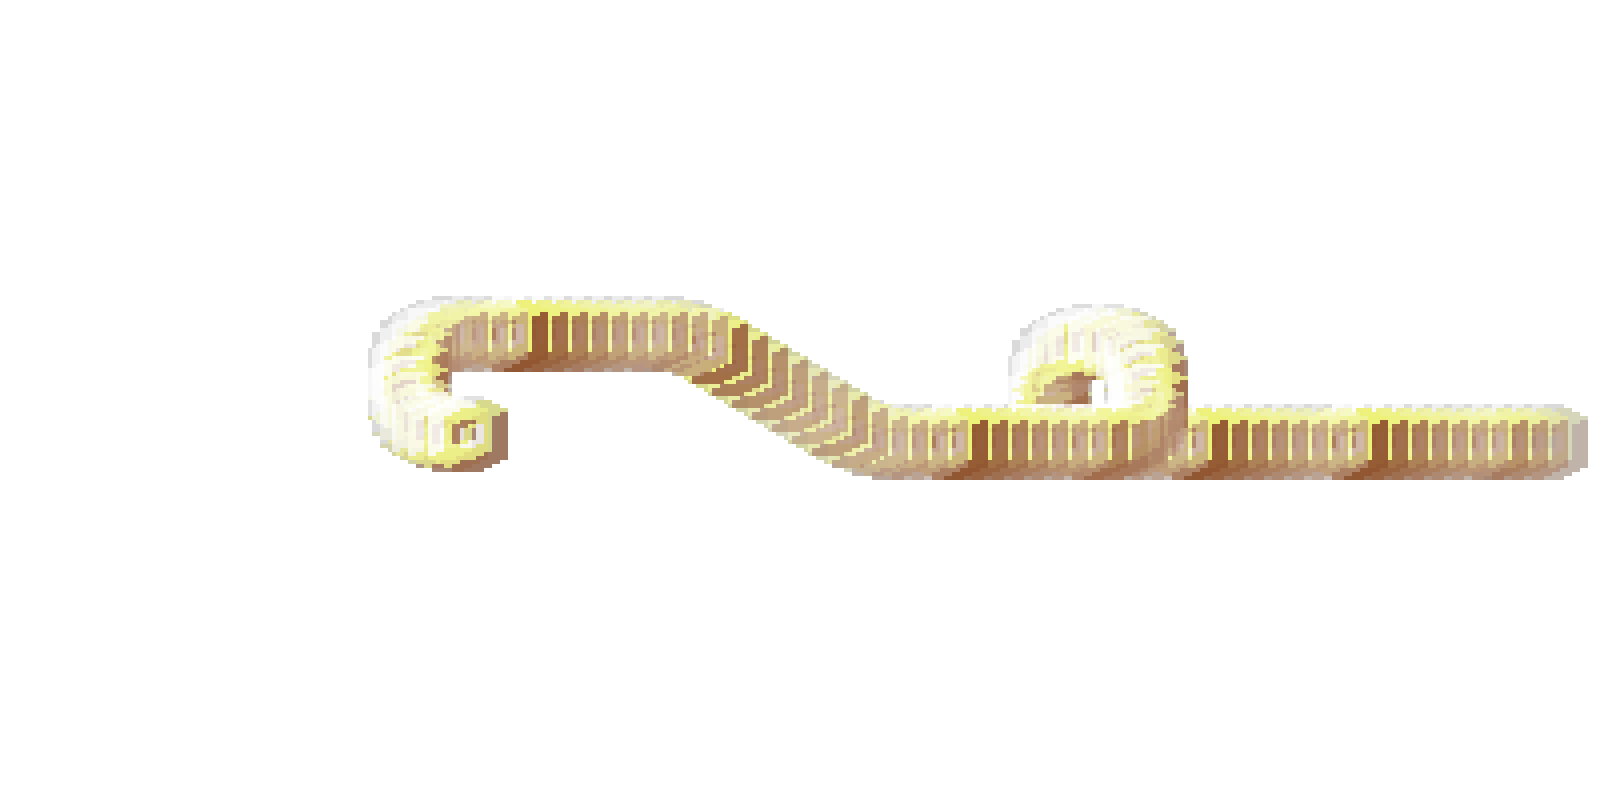
\includegraphics{src/formation_movement/strategies/strategies_17_12.png}%
		\end{adjustbox}
	\end{figure}
	\vspace{-3.4cm}
	\begin{figure}[H]
		\centering
		\begin{adjustbox}{width=7.0cm,right}
			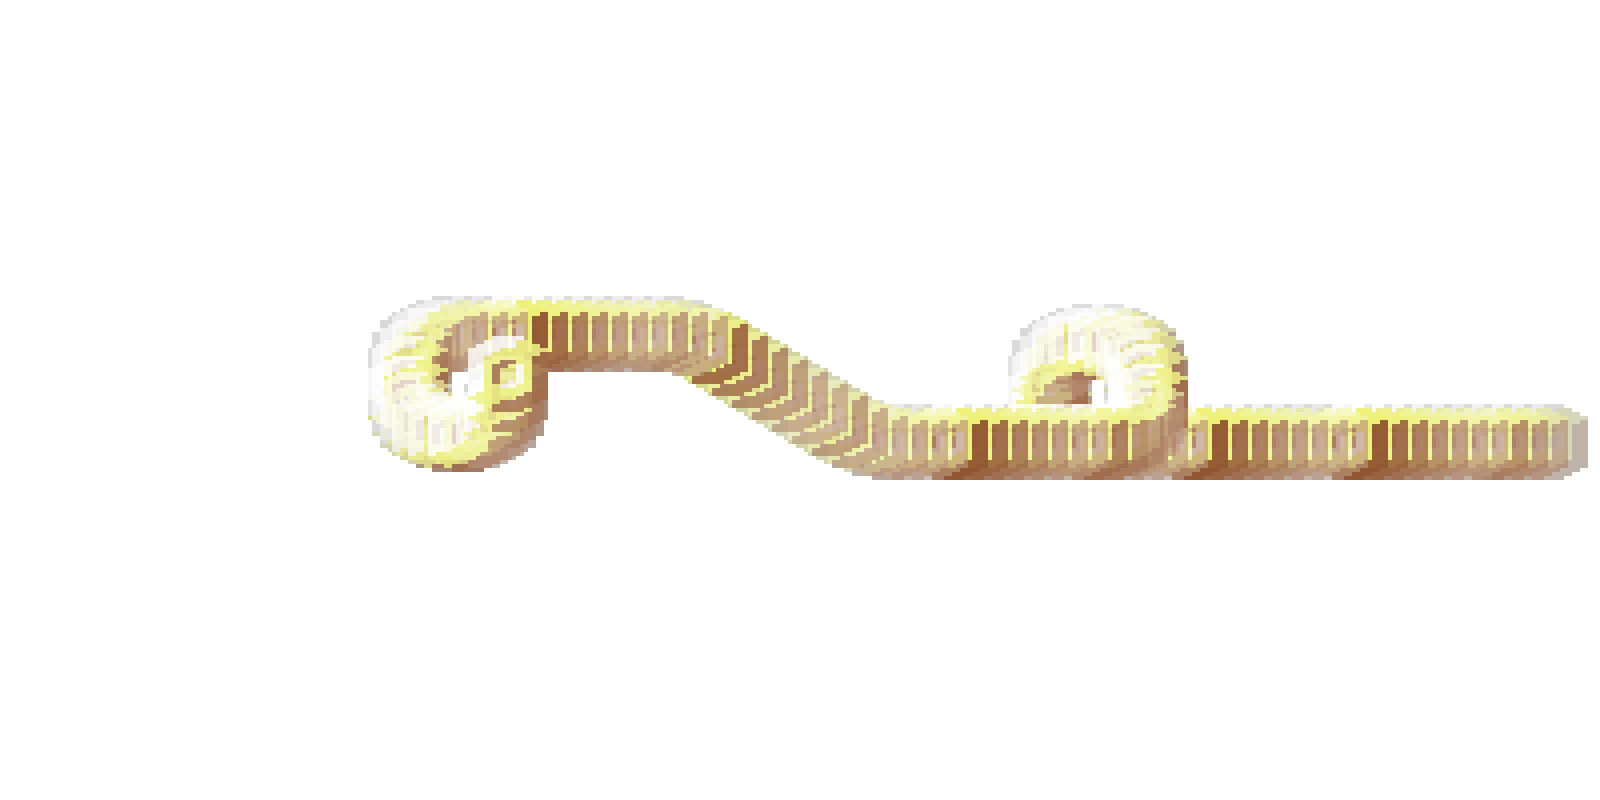
\includegraphics{src/formation_movement/strategies/strategies_17_13.png}%
		\end{adjustbox}
	\end{figure}
	\vspace{-3.4cm}
	\begin{figure}[H]
		\centering
		\begin{adjustbox}{width=7.0cm,right}
			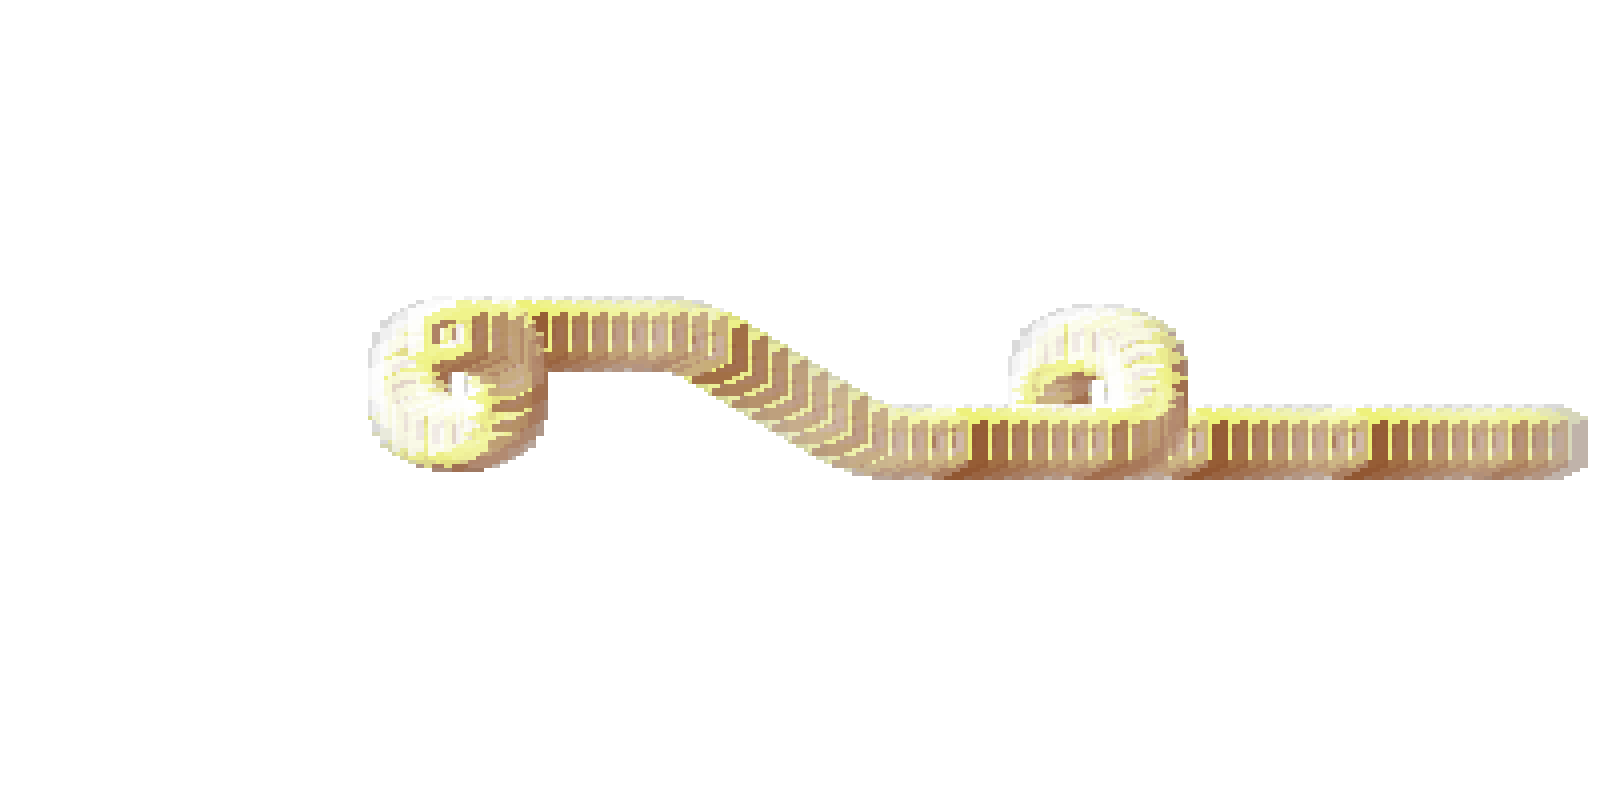
\includegraphics{src/formation_movement/strategies/strategies_17_14.png}%
		\end{adjustbox}
	\end{figure}
	\vspace{-3.4cm}
	\begin{figure}[H]
		\centering
		\begin{adjustbox}{width=7.0cm,right}
			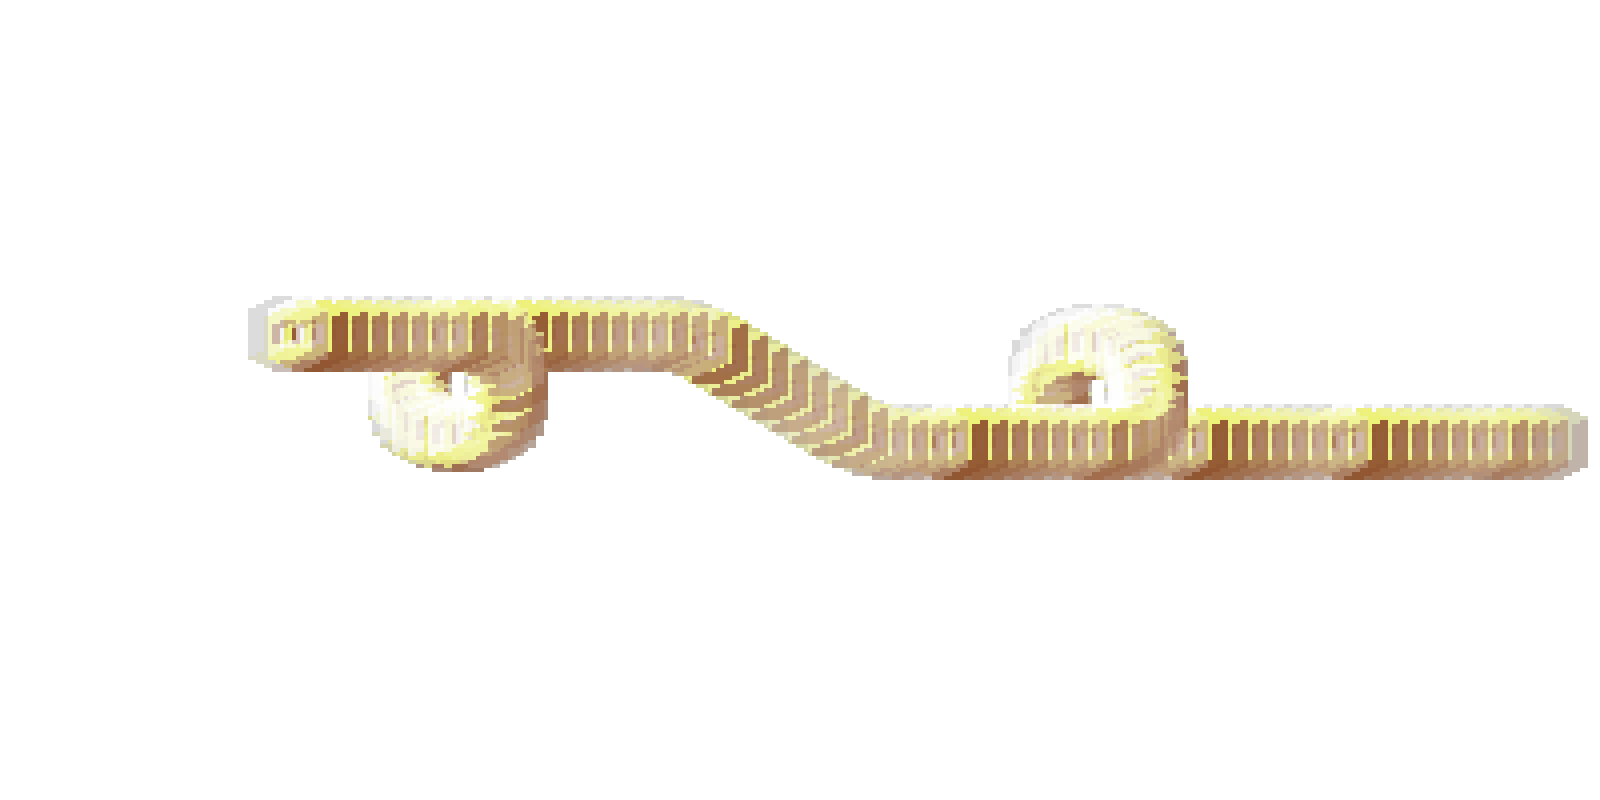
\includegraphics{src/formation_movement/strategies/strategies_17_15.png}%
		\end{adjustbox}
	\end{figure}
\end{minipage}
\hspace{0.2cm}
\vspace{-1.0cm}
\begin{minipage}[c]{0.48\linewidth}
	\vspace{-2.0cm}
\begin{lstlisting}[basicstyle=\footnotesize\ttfamily]
.BYTE $82 ; Move forward.
.BYTE $08 ; Repeat for 8 ticks.
                                 
.BYTE $80 ; Maintain movement.
.BYTE $28 ; Repeat for 40 ticks.

.BYTE $89 ; Move up and back.
.BYTE $0A ; Repeat for 10 ticks.

.BYTE $85 ; Move down and back.
.BYTE $0A ; Repeat for 10 ticks.

.BYTE $86 ; Move down and forward.
.BYTE $0A ; Repeat for 10 ticks.

.BYTE $8A ; Move up and forward.
.BYTE $0A ; Repeat for 10 ticks.

.BYTE $80 ; Maintain movement.
.BYTE $14 ; Repeat for 20 ticks.

.BYTE $88 ; Move up.
.BYTE $06 ; Repeat for 6 ticks.

.BYTE $80 ; Maintain movement.
.BYTE $0C ; Repeat for 12 ticks.

.BYTE $84 ; Move down.
.BYTE $06 ; Repeat for 6 ticks.

.BYTE $80 ; Maintain movement.
.BYTE $14 ; Repeat for 20 ticks.

.BYTE $85 ; Move down and back.
.BYTE $0A ; Repeat for 10 ticks.

.BYTE $89 ; Move up and back.
.BYTE $0A ; Repeat for 10 ticks.

.BYTE $8A ; Move up and forward.
.BYTE $0A ; Repeat for 10 ticks.

.BYTE $86 ; Move down and forward.
.BYTE $0A ; Repeat for 10 ticks.

.BYTE $00
.BYTE $FF ; Terminal pair.

\end{lstlisting}
\end{minipage}

altering its movement. We have an even more elaborate example of this
instruction stream in the diagram above: a vertical loop manouevre that we
encounter in the first level of the game. Here we notice that it is possible to
combine both X and Y axis information in our instructions. The instruction
\icode{\$89}, for example, instructs the guidance engine to alter the speed
both up and back. The instruction \icode{\$85},
meanwhile, adjusts the direction down and back. With just four byte-pairs we
can achieve a single loop, and if we look closely we can see that each loop
is accomplished using a complementary sequence of pairs.

This is hopefully giving us an idea of how \textit{Uridium} implements and encodes
the movement of the player's enemies. To continue our example, we can now see how 
defining a single movement such as this one can then be utilized to give shape
to an entire formation.

\begin{figure}[H]
  \centering
  \begin{adjustbox}{width=13.0cm,center}
    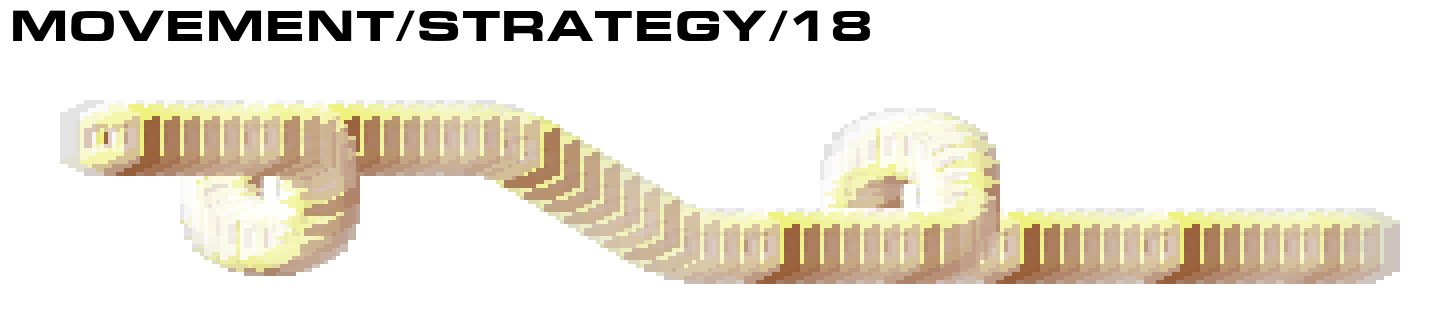
\includegraphics{src/formation_movement/strategy_diagrams/strategies_17.png}%
  \end{adjustbox}
\end{figure}
\vspace{-0.6cm}

In the second wave of Level 1 we find the above movement adopted for all members
of the formation. Notice how the 'Movement Strategy' specified for each enemy is the
one we have defined above: strategy '18'.
\begin{figure}[H]
  \centering
  \begin{adjustbox}{width=13.0cm,center}
    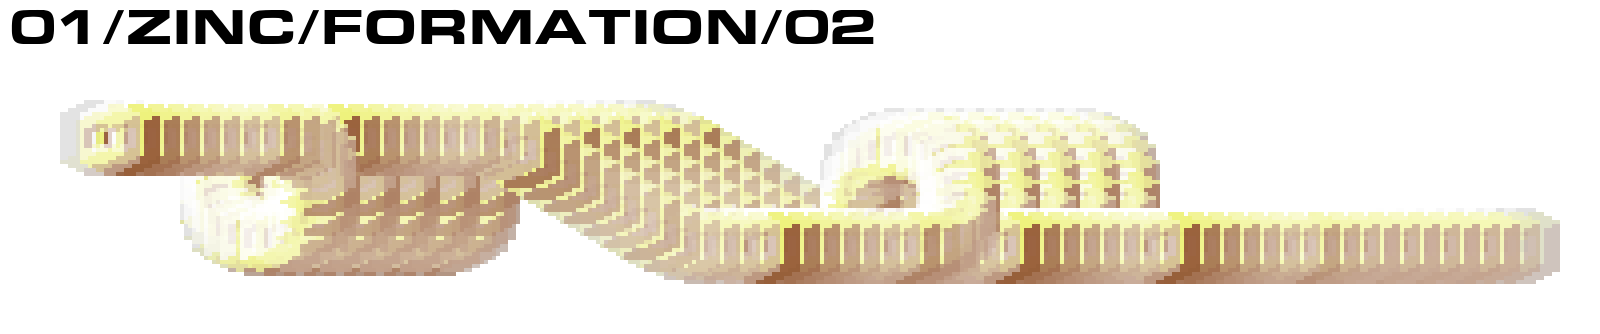
\includegraphics{src/formation_movement/level_formation_diagrams/1_formation_movement_1_25.png}%
  \end{adjustbox}
\end{figure}
\vspace{-0.8cm}
\begin{lstlisting}
enemyFormationData26
  .BYTE  18  ; Movement Strategy 18: Enemy 1
  .BYTE  18  ; Movement Strategy 18: Enemy 2
  .BYTE  18  ; Movement Strategy 18: Enemy 3
  .BYTE  18  ; Movement Strategy 18: Enemy 4
  .BYTE  18  ; Movement Strategy 18: Enemy 5
  .BYTE $00  ; Movement Strategy 18: Enemy 6
  .BYTE $CC  ; Initial Y Position : Enemy 1
  .BYTE $CC  ; Initial Y Position : Enemy 2
  .BYTE $CC  ; Initial Y Position : Enemy 3
  .BYTE $CC  ; Initial Y Position : Enemy 4
  .BYTE $CC  ; Initial Y Position : Enemy 5
  .BYTE $00  ; Initial Y Position : Enemy 6
  .BYTE $05  ; Delay between spawning enemies.
  .BYTE $80  ; Initial X Position of Enemy 1
  .BYTE $08  ; Sprite Value for Enemies
  .BYTE $00  ; End Sentinel
\end{lstlisting}

We encountered these definitions in the previous section, but had remained silent on the meaning of these
'Movement Strategies'. Now their purpose has become apparent. Notice how the dynamic of the formation
depends on each of the enemies arriving at the same vertical position, one after the other like a train, and
how the interval is definte by the 'Delay between spawning enemies'. This compact description, in tandem
with the instruction stream for the movement strategy, is enough to create a powerful effect, like an implacable
enemy force barrelling across the player's view.

We find variations on this theme used in later levels, such as 'Quadmium', where we find interlocking vertical loops
expanding to cover a larger expanse - posing a greater threat to the player.
\begin{figure}[H]
  \centering
  \begin{adjustbox}{width=13.0cm,left}
    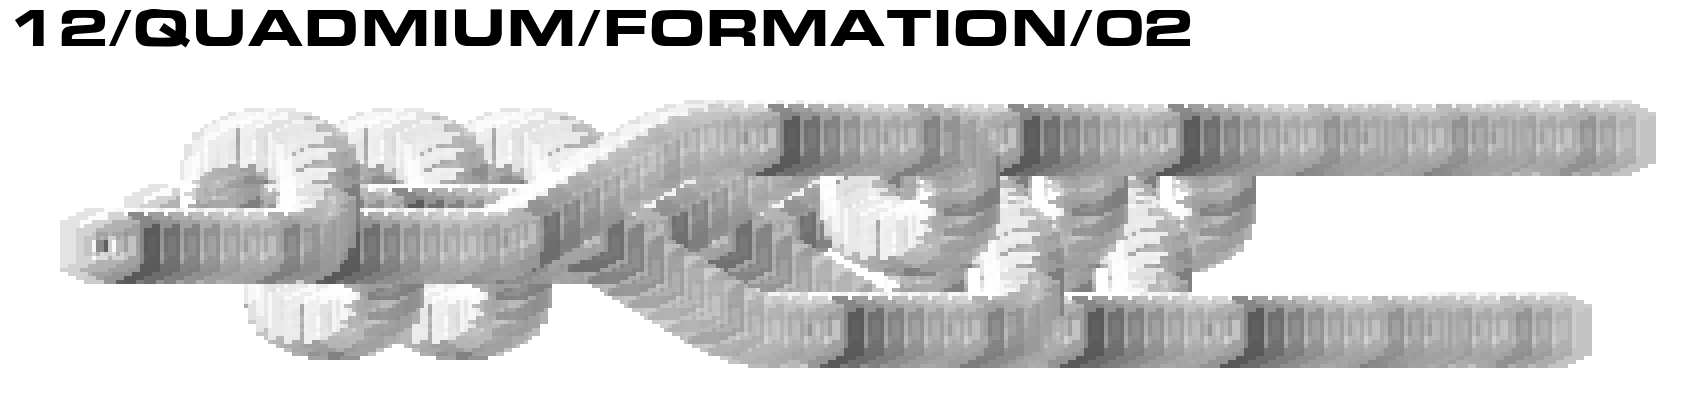
\includegraphics{src/formation_movement/level_formation_diagrams/12_formation_movement_1_28.png}%
  \end{adjustbox}
\end{figure}
\vspace{-0.6cm}

Visualizing the level formations in this way creates some pleasing artefacts, particularly where there
is a diverse set of movement strategies in play. In this example from Level 5 (\textit{Iron}), enemies
pass across each other performing some loosely co-ordinated maneouvres in the center of the screen. The
final effect resembles a toy rail network.

\begin{figure}[H]
  \centering
  \begin{adjustbox}{width=13.0cm,left}
    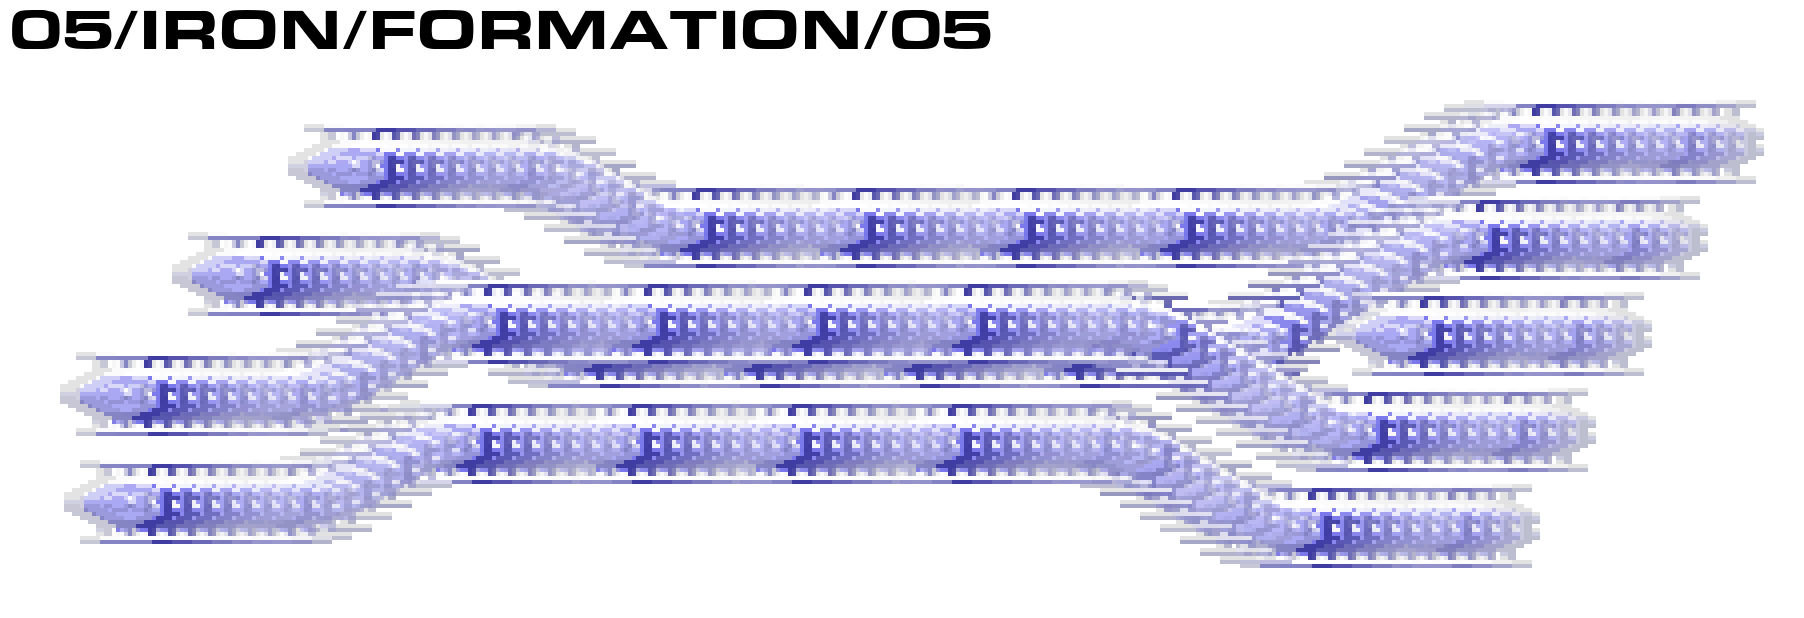
\includegraphics{src/formation_movement/level_formation_diagrams/5_formation_movement_4_55.png}%
  \end{adjustbox}
\end{figure}
\vspace{-0.6cm}

In Level 6 (\textit{Gold}), we find a more twisted configuration. This specimen is utilising variations
on the very first movement strategy we looked at, a rapid slalom that deviates from their heading before
quickly resuming it. Notice how the different starting positions, along with only two variations on the
slalom maneouvre, combine to create a twisted nest of flight patterns.

\begin{figure}[H]
  \centering
  \begin{adjustbox}{width=13.0cm,left}
    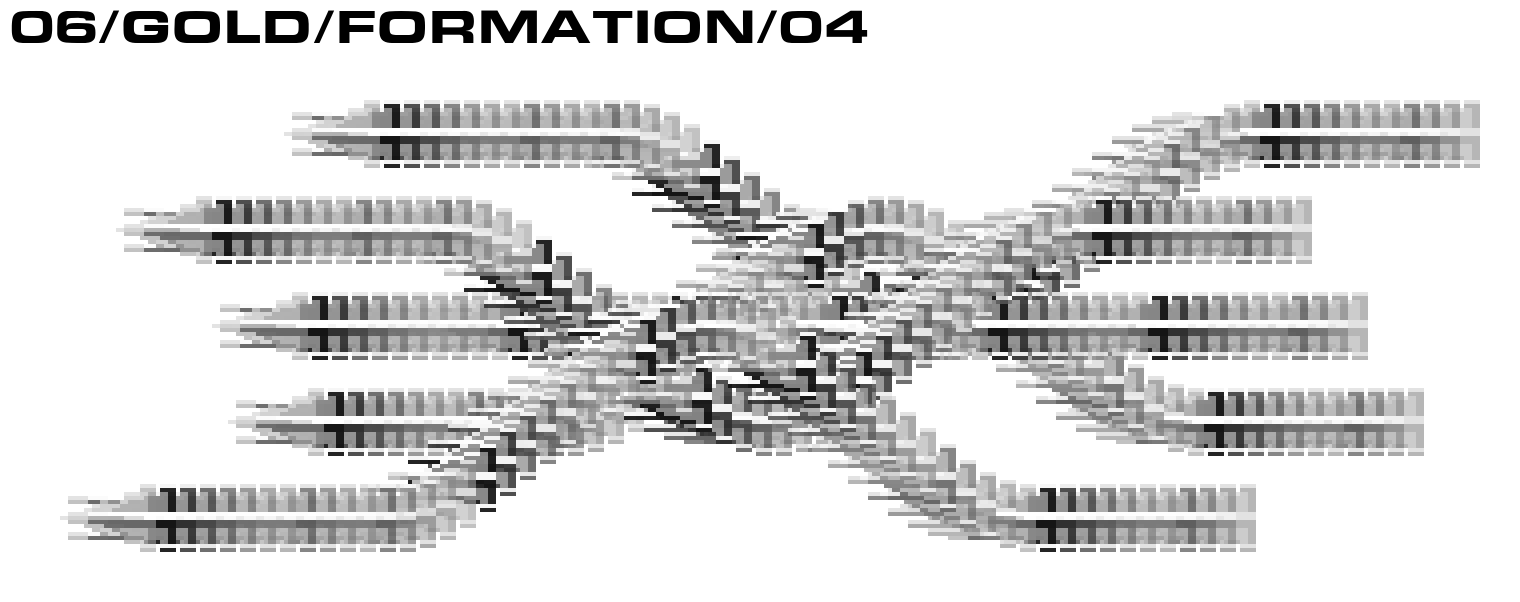
\includegraphics{src/formation_movement/level_formation_diagrams/6_formation_movement_3_44.png}%
  \end{adjustbox}
\end{figure}

Our final example on the opposite page shows us what may really be at work with these sinuous flightpaths.
Halfway through a simple horizontal heading the enemies spin off and disappear from view. This means the player
must act fast in order to shoot them. This reinforces our suspicion that these elaborate movement strategies
are above all evasive maneouevres designed to make it as difficult as possible for the manta to get a bead
on them and destroy them. The deviations in their path always occur just as the player might have adjusted
their position to meet them head on. 

\begin{figure}[H]
  \centering
  \begin{adjustbox}{width=13.0cm,left}
    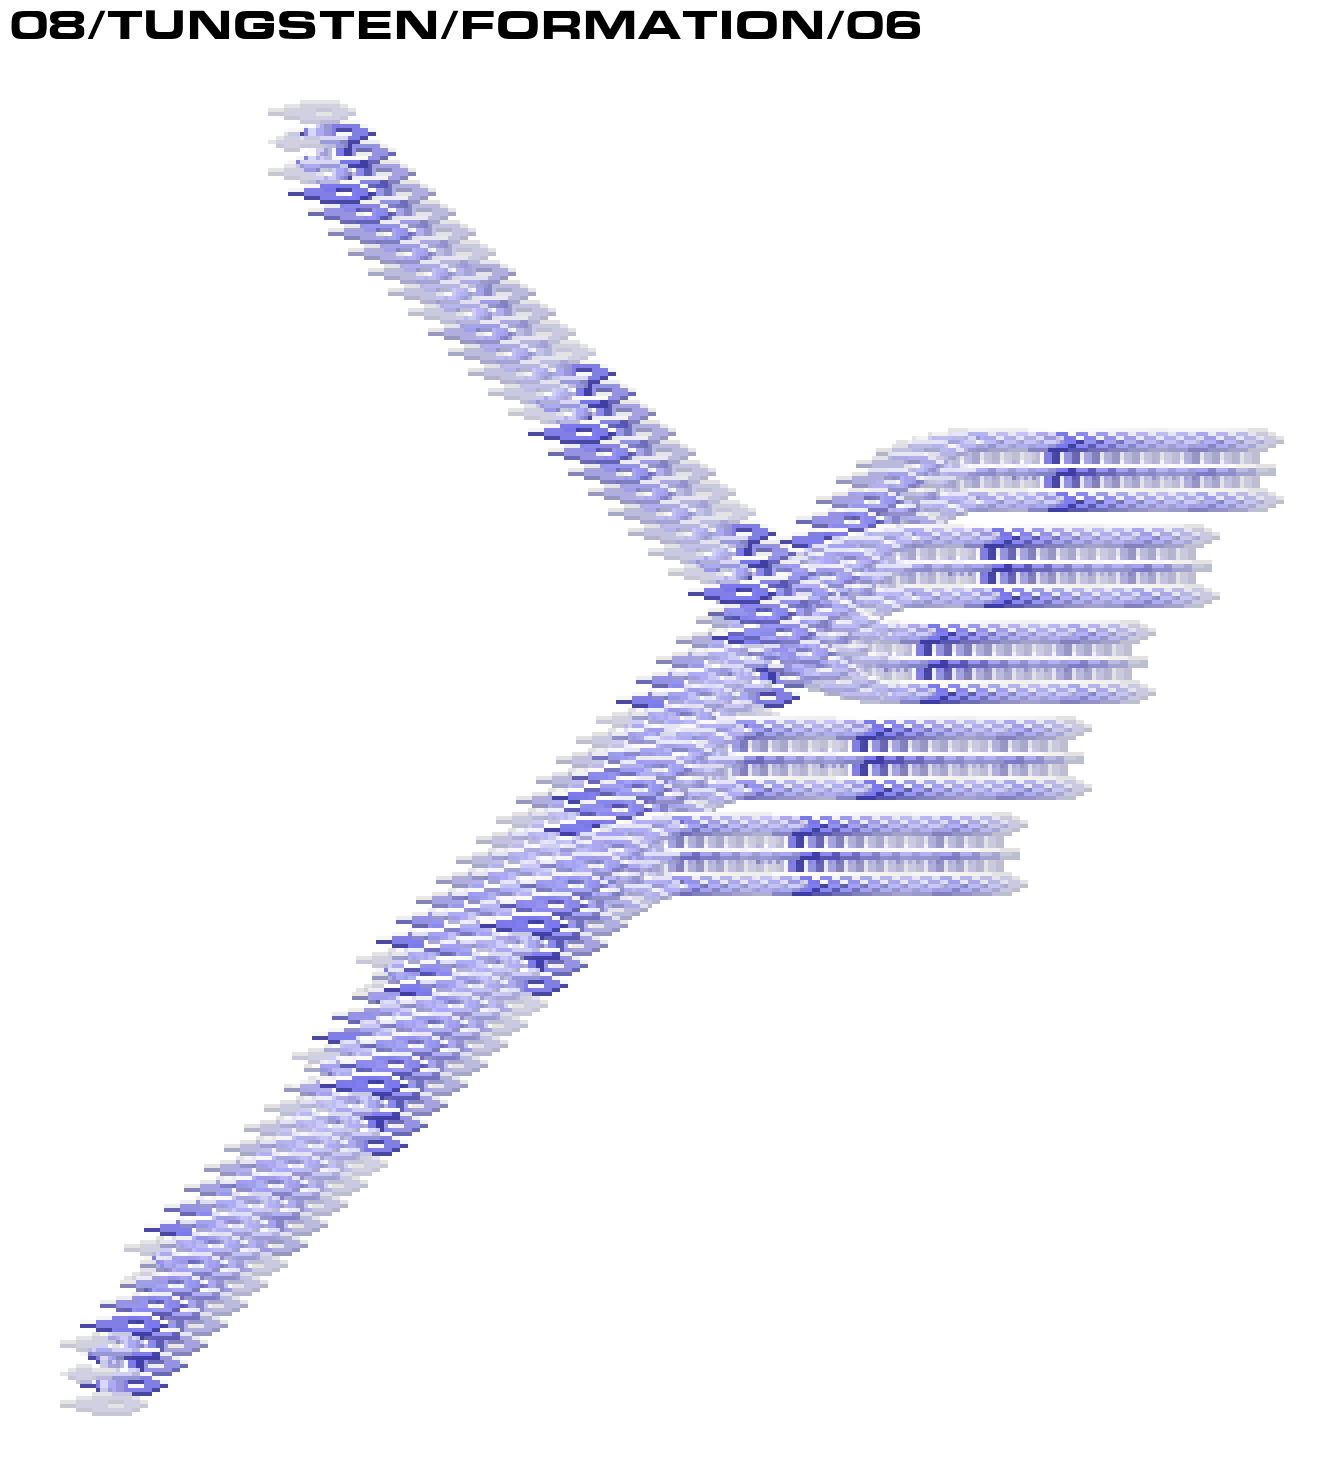
\includegraphics{src/formation_movement/level_formation_diagrams/8_formation_movement_5_29.png}%
  \end{adjustbox}
\end{figure}



%\clearpage
%\begin{minipage}[c]{0.43\linewidth}
%	\vspace{-1.6cm}
%	\begin{figure}[H]
%		\centering
%		\begin{adjustbox}{width=7.0cm,right}
%			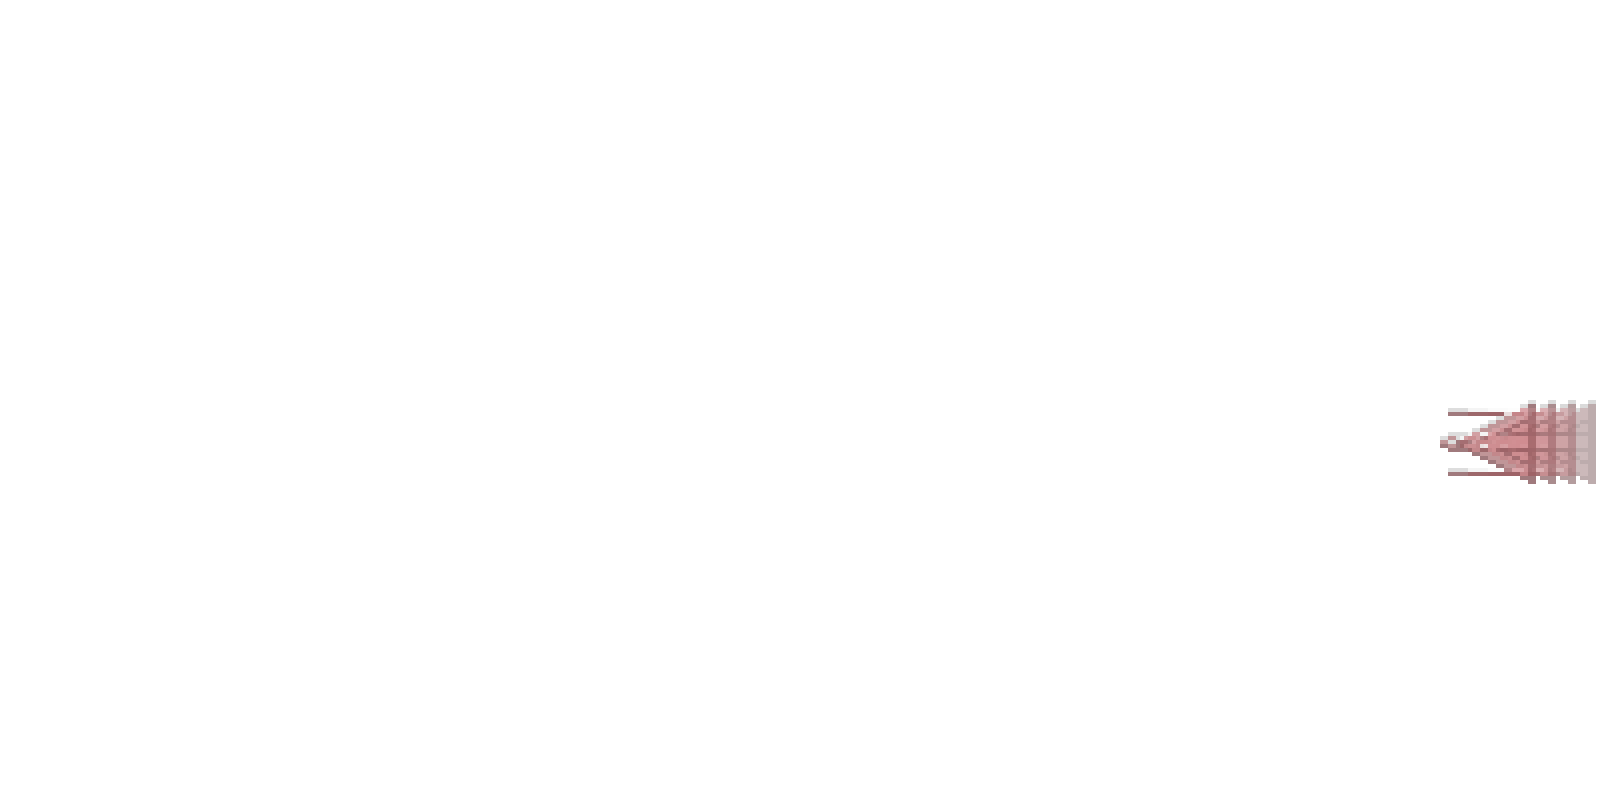
\includegraphics{src/formation_movement/strategies/strategies_28_0.png}%
%		\end{adjustbox}
%	\end{figure}
%	\vspace{-3.3cm}
%	\begin{figure}[H]
%		\centering
%		\begin{adjustbox}{width=7.0cm,right}
%			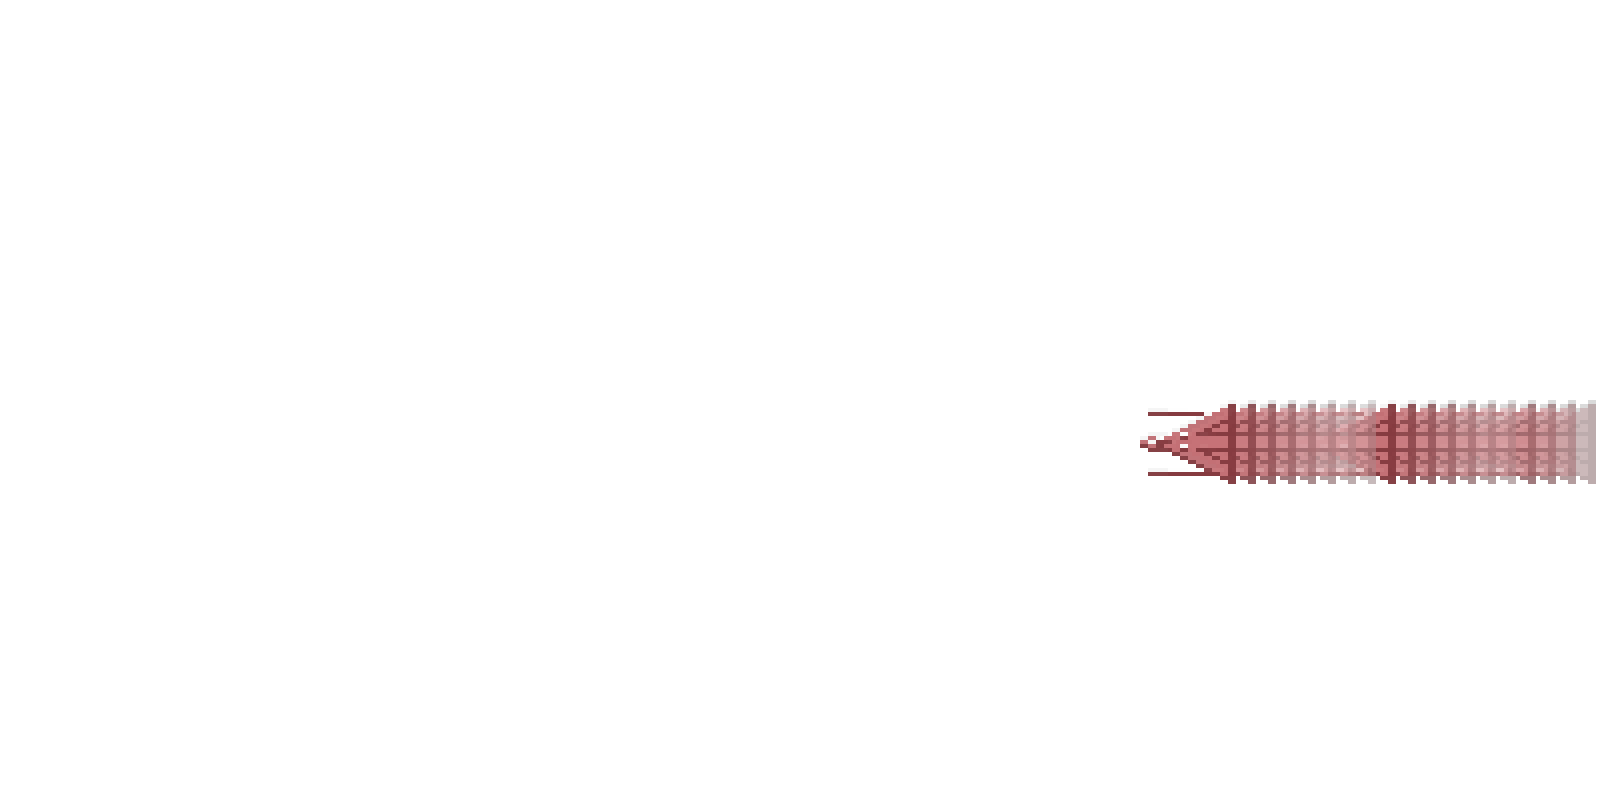
\includegraphics{src/formation_movement/strategies/strategies_28_1.png}%
%		\end{adjustbox}
%	\end{figure}
%	\vspace{-3.3cm}
%	\begin{figure}[H]
%		\centering
%		\begin{adjustbox}{width=7.0cm,right}
%			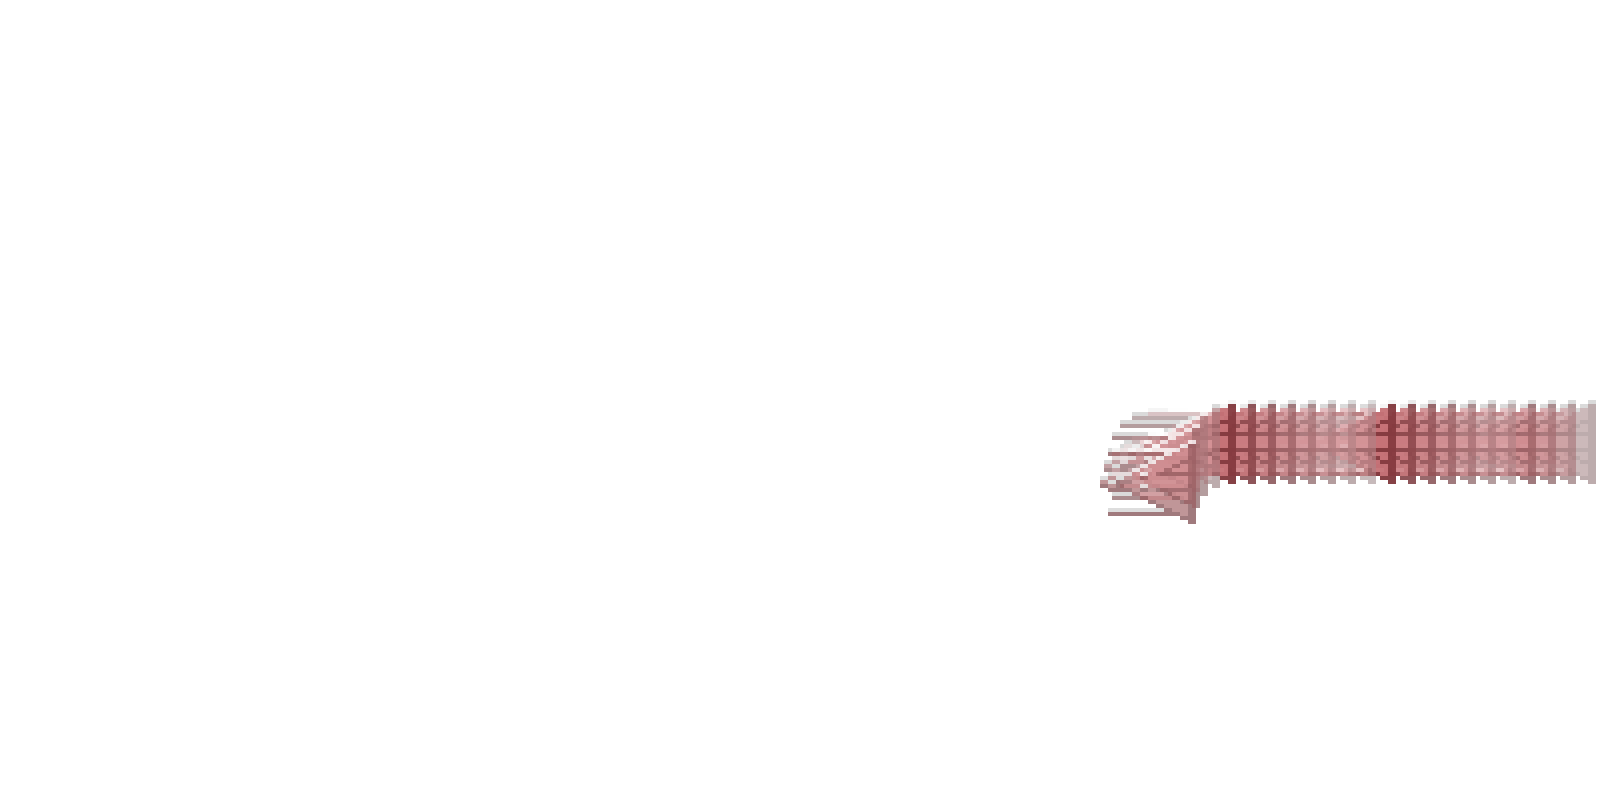
\includegraphics{src/formation_movement/strategies/strategies_28_2.png}%
%		\end{adjustbox}
%	\end{figure}
%	\vspace{-3.3cm}
%	\begin{figure}[H]
%		\centering
%		\begin{adjustbox}{width=7.0cm,right}
%			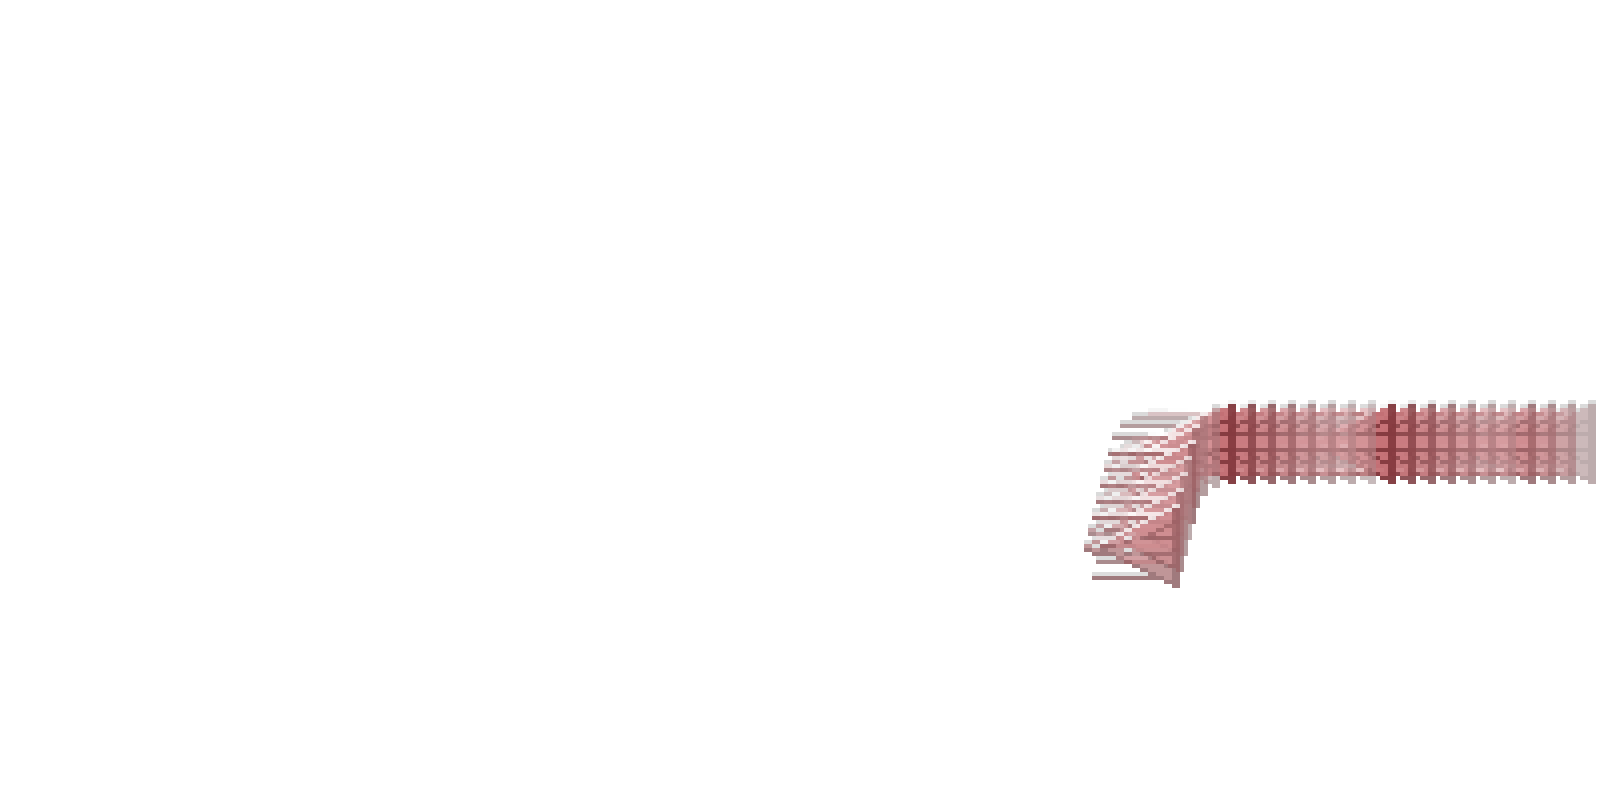
\includegraphics{src/formation_movement/strategies/strategies_28_3.png}%
%		\end{adjustbox}
%	\end{figure}
%	\vspace{-3.3cm}
%	\begin{figure}[H]
%		\centering
%		\begin{adjustbox}{width=7.0cm,right}
%			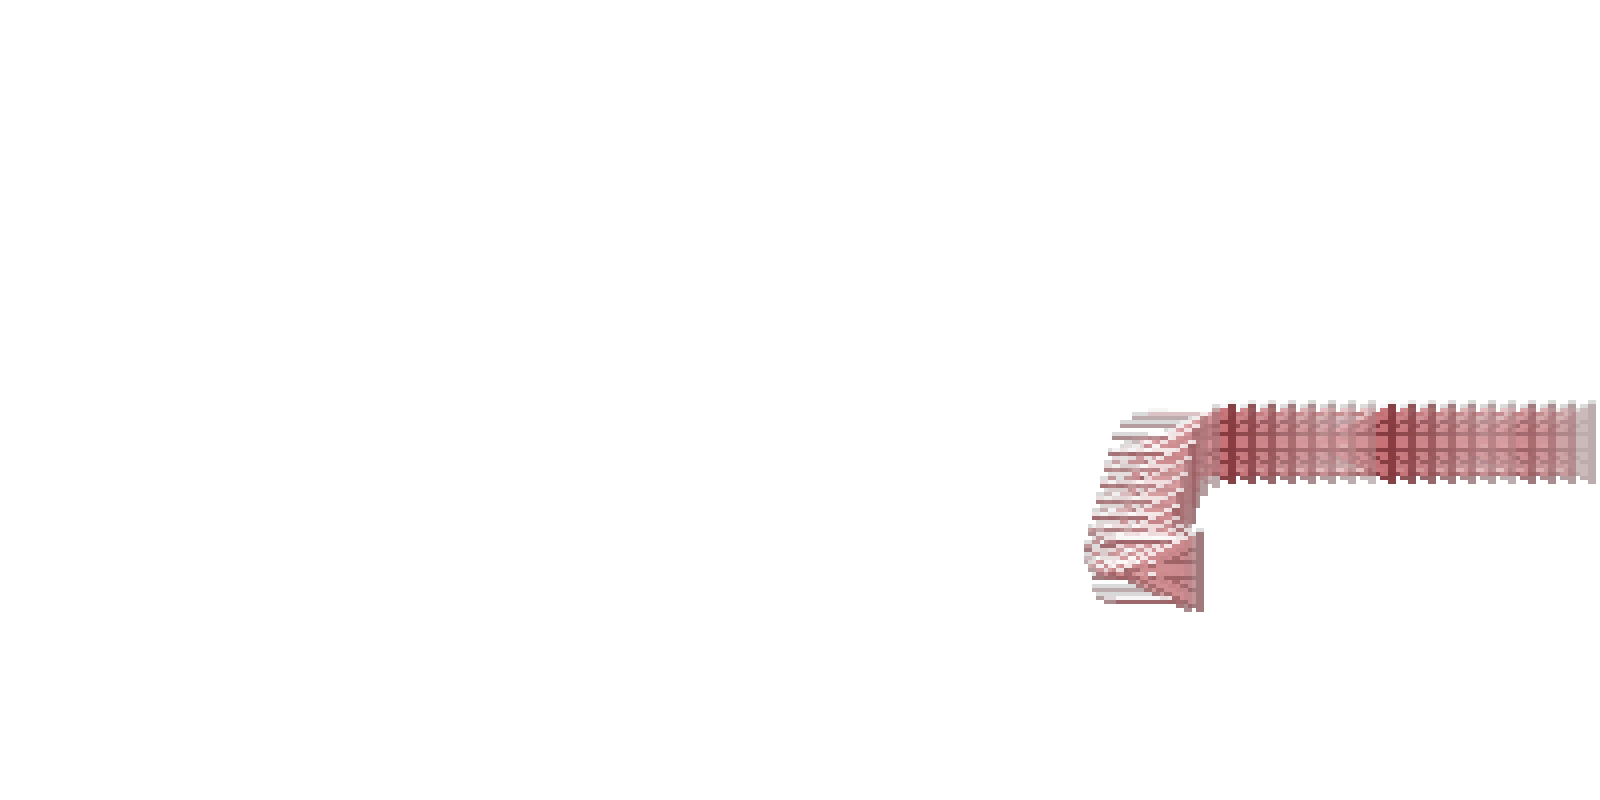
\includegraphics{src/formation_movement/strategies/strategies_28_4.png}%
%		\end{adjustbox}
%	\end{figure}
%	\vspace{-3.2cm}
%	\begin{figure}[H]
%		\centering
%		\begin{adjustbox}{width=7.0cm,right}
%			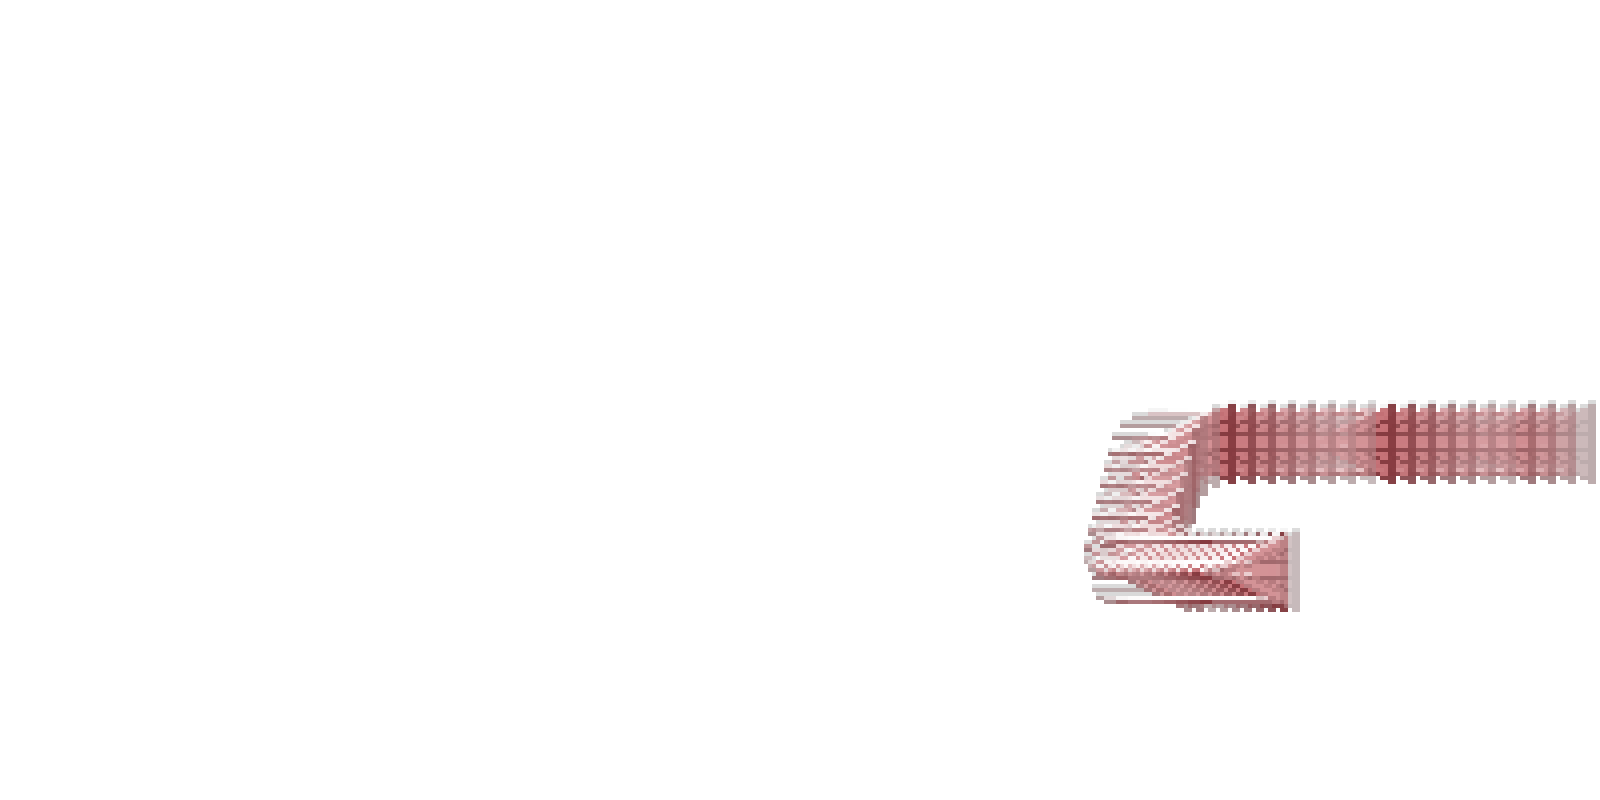
\includegraphics{src/formation_movement/strategies/strategies_28_5.png}%
%		\end{adjustbox}
%	\end{figure}
%\end{minipage}
%\begin{minipage}[c]{0.58\linewidth}
%	\vspace{-1.0cm}
%\begin{lstlisting}[basicstyle=\footnotesize\ttfamily]
%.BYTE $82 ; Move forward.
%.BYTE $08 ; Repeat for 8 ticks.
%                                   
%.BYTE $80 ; Maintain movement.
%.BYTE $24 ; Repeat for 36 ticks.
%                                   
%.BYTE $85 ; Move down and back.
%.BYTE $08 ; Repeat for 8 ticks.
%                                   
%.BYTE $80 ; Maintain movment.
%.BYTE $02 ; Repeat for 2 ticks.
%                                   
%.BYTE $89 ; Move up and back.                         
%.BYTE $08 ; Repeat for 8 ticks.
%
%.BYTE $00
%.BYTE $FF ; Terminal pair.
%\end{lstlisting}
%\end{minipage}
